% Created 2017-03-23 Thu 11:37
% \documentclass[11pt]{article}
\documentclass[twocolumn,10pt]{article}
\usepackage[utf8]{inputenc}
\usepackage[T1]{fontenc}
\usepackage{fixltx2e}
\usepackage{graphics}
\usepackage{subfig}
\usepackage{grffile}
\usepackage{longtable}
\usepackage{wrapfig}
\usepackage{rotating}
\usepackage[normalem]{ulem}
\usepackage{amsmath}
\usepackage{textcomp}
\usepackage{amssymb}
\usepackage{capt-of}
\usepackage{hyperref}
\usepackage[section]{placeins}
\input asl_setup.tex
\newcommand {\srf}  {\mbox{\small SRF}}
\setlist{itemsep=2pt,parsep=-1pt,partopsep=0pt} %,topsep=0pt}
\geometry{letterpaper,textwidth=7in,textheight=9.3in}
\titlespacing{\subsubsection}{0pt}{10pt plus 2pt minus 2pt}{2pt plus 2pt minus 2pt}
\author{chris hepplewhite et al.}
\date{\today}
\title{A Hyper-Spectral Multi-Sensor Infrared Radiance Data Record for Climate Trending: \\  
  Validation using Simultaneous Nadir Observations \\  
  \vspace{3mm}
  {****} DRAFT {****}\\
}

\hypersetup{
 pdfauthor={chris hepplewhite},
 pdftitle={},
 pdfkeywords={},
 pdfsubject={},
 pdfcreator={Emacs 25.1.1 (Org mode 8.3.6)}, 
 pdflang={English}}
\begin{document}
\maketitle

%\tableofcontents

\section{Abstract.}

A long term hyper-spectral radiance record using multiple sensors for climate monitoring is proposed. This is achieved by converting the spectral radiance measurements to a common response function. The considerable overlap of three operational satellite-based weather missions is used to accumulate a large statistically significant data set from which to study the bias and error characteristics of the sensor records and the conversion method.

The conversion of the radiance measurements from AQUA-AIRS (Atmospheric Infrared Sounder), Suomi-NPP CrIS (Cross-track Infrared Sounder) and MetOp IASI (Infrared Atmospheric Sounding Interferometer) to a common spectral grid is described and validated. The common grid adopted here is that used by the nominal CrIS instrument. The goal with the current sensors is to produce a radiance climate record from September 2002 well into the future, currently representing 14+ years, for studying climate trends and anomalies.

The conversion of the radiance spectra from one spectral grid to another is detailed in a companion paper. The method is validated using simulations from standard atmospheric profiles and a fast high-resolution forward model. A considerable advantage of this method over others is that trends and anomalies in top-of-atmosphere radiance can be obtained over a large spectral range in the thermal infra-red at high spectral resolution.

The principal method used to validate the combined data set is with very large samples of simultaneous nadir overpass (SNO) observations. From these, the biases and stability characteristics of the sensors and any dependencies on the SNO scenes are determined.

We evaluate clearly traceable uncertainties to the final estimates from which a common radiance record is derived. Over much of the spectral and dynamic range of the sensors studied, this method resolves the bias between sensors with a precision of about 10 mK. The actual bias between sensors is found to be dependent upon the frequency and brightness temperature of the scene, the details are found in the sections below.


\section{Introduction}

The research summarized in this paper describes the foundation of a method for producing a continuous climate quality radiance record from the hyper-spectral infra-red measurements obtained from low-Earth orbiting (LEO) satellites by translating the radiance observations on to a common wavenumber scale.

Detection of climate change signals requires long-term, highly accurate measurements with optimal spatial coverage, for example \cite{wielicki2013} and for a period of time sufficiently long so as to distinguish natural internal variations. The long-term calibration and spectral stability of observation systems are essential for the reliable detection of climate variations. The spatio-temporal resolution and coverage of the measurements should be representative of the true state of the atmosphere. Whereas ground based observation systems are generally well calibrated, they tend to observe regionally and not globally. Satellite observing systems provide the global coverage and their calibration is much improved recently. The challenge now is to demonstrate that current satellite sensor technologies are suitable for this task.

It is important to distinguish between internal climate variability and external forcing \cite{solomon2010}. Internal variations of interest include, but are not limited to, the El Nino Southern Oscillation (ENSO), the Pacific Decadal Oscillation (PDO) and Atlantic multi-decadal oscillation (AMOC). External factors include, but not limited to human activities and industrial processes, Solar changes, asteroids and volcanic erruptions \footnote{the convention is to refer to internal variability for atmospheric and oceanic processes. }. See for example, the IPCC (Intergovernmental Panel on Climate Change) assessment report 4, working group 1 and references therein \cite{ipcc2007_wg1}. 

There are a variety of essential climate variables (ECVs) that are used to monitor the state of the climate, see for example the World Meteorological Organisation (WMO) Global Climate Observing System (GCOS), reference \cite{gcos}. As described therein, the dynamic range, resolution and absolute calibration accuracy required to properly record the variable being measured are delineated. The approach taken here is to use the spectral radiance measured by several sensors, over a range of infrared wavelengths that are sensitive to these ECVs to monitor the state of the climate.

There are a large variety of sensors being used to measure the ECVs, see ref \cite{Hollmann2013} and new ones are being deployed to augment or replace old sensors.  Since around the turn of the 21st century, improved technologies have resulted in more stable sensors and longer periods of observations with the same sensor, furthermore, new ones have been deployed so there is a substantial overlap. This helps to produce a meaningful climate quality data record. Nevertheless, the sensors and the observational sampling are not identical, and so it is necessary to develop new techniques to analyze and merge the data sets to obtain a product that can be used for climate monitoring and research.

When working with the observations from different, but similar sensors, great care must be taken to understand and quantify the statistical characteristics of the data and the detail of the scenes being observed and any dependencies thereon. Different strategies have been adopted to compare the different sensors, for example, refer to \cite{Chander2013} for an excellent overview and references therein. In this work simultaneous nadir observations (SNOs) are best suited to comparing the AIRS and CrIS sensors because of their similar viewing geometry, orbit and spectral coverage. The SNO methodology has been employed for many years and for many different sensors, sometimes direct differencing \cite{Wang2007} and double differencing, \cite{Wang2011}, and even when the spectral bands are different, \cite{Uprety2013}. In the case of the comparison between Aqua AIRS and Metop-IASI, where the geographical converage of the SNOs is limited, see for example \cite{GSICS2008}, the dynamic range is similarly restricted. In \cite{Elliott2009} only a small number of channels are considered but the authors use ECMWF modelled radiances as a transfer standard for studying double differences. In this work SNOs for AIRS, CrIS and IASI are used to take advantage of the strengths of each combination.

In order to compare the measured signal from different sensors the spectral content of the radiance must be comparable. If the two sensors have identical spectral response functions then this is achieved by definition. In general for infrared hyperspectral sensors with spectral resolution similar or finer than pressure broadened emission/absorption lines of atmospheric gases, there will not be sufficient correspondance of channels between the two sensors. Different methods have been attempted that take advantage of features of the emission spectra and sensor bandwidth, for example in \cite{Wang2015} the radiance for AIRS, IASI and CrIS are compared by selecting 25 spectral bands each of which include several channels, and averaging for samples of SNOs. In the work of \cite{Ciren2003} AIRS and HIRS radiances are compared using a simple convolution of selected AIRS channels onto the HIRS channels. These methods were more rigorously employed in the work of \cite{Wang2007} where several AIRS channels are convolved into the much broader HIRS channel for the SNO samples. The spectral radiance of CrIS and IASI can be compared over the common spectral band using conventional deconvolution methodology, for example, \cite{Wang2015}.

In this work the conversion of radiances from one spectral grid to another is extended to include deconvolution of the AIRS channels to the CrIS channels on a common spectral band. Details of this method are described in a companion paper \cite{Motteler2017a} and an overview of the method and a summary of its validation is provided below. 

The following sections first describe the sensors and observations available to us; then the method for translating the observations, then the validation of the methods using SNO pairs with a discussion of results, conclusions and suggestions for further work.

\section{Observations}

The sensors used in this study are the Atmospheric InfraRed Sounder (AIRS) on the NASA EOS Aqua satellite, the Cross-track Infrared Sounder (CrIS) on the Suomi-NPP satellite and the Infrared Atmospheric Sounding Interferometer (IASI) on the European Metop satellite.

In brief summary, AIRS is an echelle grating spectrometer covering the spectral range from 3.74 to 4.61 $\mu m$ , from 6.20 to 8.22 $\mu m$, and from 8.8 to 15.4 $\mu m$, with nominal spectral resolution $\lambda/\delta\lambda= 1200$ using a total of 2378 spectral channels. The details of the spectral response functions are available, for example see reference \cite{airscalib}. AIRS is mounted on the NASA EOS Aqua spacecraft which is in a LEO sun-synchronous orbit with 98 degree inclination and equator crossing about 1:30pm. AIRS is a nadir sounder with a lateral scanning mirror that provides 90 footprints from about 45 degree either side of nadir. The footprints are about 13.5 km diameter at nadir. For more details see reference \cite{airseos}. The data used for this work are the level 1b geolocated calibrated radiances, which are further processed to level 1c for conversion, see below.

The CrIS sensor is a Michelson interferometer with 1305 channels covering the spectral range in three sub-bands from 3.92 to 4.64 $\mu m$, 5.71 to 8.26 $\mu m$ and 9.13 to 15.3 $\mu m$ referred to as the short, medium and long (SW, MW and LW resp.) sub-bands. When first launched, the spectral resolution in each sub-band was different with LW: 0.625 cm$^{-1}$, MW: 1.25 cm$^{-1}$, SW: 2.5 cm$^{-1}$, but since December 2014 all bands operate with 0.625 cm$^{-1}$ resolution. CrIS is mounted on the Suomi-NPP weather satellite, also in a LEO, sun-synchronous, 98-degree inclination orbit and 1:30 pm equator crossing time. The Suomi-NPP orbit altitude is about 100 km higher than AQUA, so it's orbit period is slightly longer. CrIS is a nadir sounder with a lateral scanning mirror that provides 30 ground views within 45 degrees either side of nadir. Each ground view consists of nine fields of view on a square grid, each with a diameter 14 km at nadir. For more details see for example references \cite{crisweb} and \cite{criscal}. The data used in this work are the geolocated calibrated radiances processed through the Interface Data Processing Segment (IDPS).

The IASI sensor is a Michelson interferometer with 8461 channels covering the spectral range from 3.62 to 15.5 $\mu m$ with a nominal resolution of about 0.5 cm$^{-1}$. IASI is mounted on the MetOp satellite, also a LEO, sun-synchronous, 98 degree inclination, with a 9:30 am equator crossing time. IASI is a nadir sounder with a lateral scanner. Each ground view consists of four fields of view on a square grid, each about 13 km diameter at nadir. There are 30 ground views within 45 degrees either side of nadir. For more details see for example references \cite{iasiweb} and \cite{iasiover}. The data used are the gelocated calibrated radiances supplied to level 1c.

AIRS has been operating since about September 2002, CrIS on Suomi-NPP since about February 2012 and IASI-1 on MetOp-A since about November 2006 and IASI-2 on Metop-B since about October 2012. There is therefore considerable temporal overlap of these missions for which comparisons can be made. At the time of writing CRIS-2 on JPSS-1 is due for launch late 2017. Note that the orbit of Metop-A has morning equator crossing whilst AQUA and Suomi-NPP are afternoon crossing which influences where the SNOs are located.

It is worth noting that there have been continuous hyperspectral infrared global atmospheric soundings since 2002, and the prospect of another decade or so with just those instruments described above. Furthermore, the spectral range, spectral resolution and spatial sampling of these sensors have similar attributes, which permits comparisons to be made rather readily. Nevertheless, differences between the sensors must be accounted for correctly.

With the relatively long and increasing data set, it is possible to relate the observations to known components of global internal climate variability and average global warming trends. There are several possible ways this can be done, including tracking levels of long-lived (passive) tracer gases, cloud amounts and surface temperature and identifying changes in the statistical distributions, such as their extremes and high-order moments for example \cite{DeSouzaMachado2017a}.

In this paper we describe the direct comparison of spectral radiance at the top of the atmosphere (TOA) as measured by the sensors. We produce a TOA spectral radiance data set with a common spectral grid and equivalent spectral response that can be used with multiple sensors to support climate studies.

The techniques used and their validation are presented in the following sections.  

\section{Methods}

This section firstly describes the techniques and methods used to generate a common set of spectral radiance channels from the individual sensors and secondly to acquire the observation data sets for the comparisons. 

\subsection{Radiance Translation and Spectral Resampling}

In this context, radiance translation refers to the conversion of the spectral radiance measurements made by one sensor to what it would be if measured by the other sensor. In general, it involves several mathematical operations including deconvolution or Fourier decomposition, depending on the original sampling type and which are referred to as spectral resampling.

In practice, the resolution of all sensors is not much different, so the choice to use the CrIS standard resolution sampling for the common spectral bands is convenient. In theory, any real or synthetic grid could be used but the resampling works better from high to low resolution. This choice may be revisited in the future, since CrIS changed to high-resolution in all three of its bands in December 2014.

Consider the idealized case in which the radiant energy received by the sensors is from a blackbody Planck emitter and it is sampled uniformly in frequency across the thermal infra-red (TIR) band, and the response function of the sensors are perfectly known. Then, the measured signal is the SRF convolved with the Planck function, and so for sensors with different spectral response functions, the source emission will be perfectly known and spectral resampling of the radiance between sensors will be equivalent, \cite{Motteler2017b}. 

In the real world, the infra-red radiance includes bands of high contrast molecular emission lines, with line-widths varying according to the height in the atmosphere. It is easy to see that each sensor will sample the emission lines differently and the signal will be dependent upon several factors including, the sampling interval, the band width and knowledge of the response functions. The translation method works well because the radiance is sampled by many overlapping SRFs, as in the case of AIRS is shown in summary below and in detail in \cite{Motteler2017a}. Uniform sampling is self evident for the CrIS and IASI interferometers, but for AIRS this is not the case. Furthermore, some AIRS channels may have failed during the course of its operation or become too noisy, so this method is dependent upon using the level 1C spectra \cite{Manning2015}, which has spectral gaps filled and faulty channels repaired. The AIRS SRFs have been determined pre-flight at 0.01 cm$^{-1}$ resolution and the intermediate grid is 0.1 cm$^{-1}$ is used.

%Suppose there are $n$ channels on a frequency grid $v$ of $k$ points spanning the domains of the %functions $\text{srf}_i$. Let $S_k$ be an $n\times k$ array such that $s_{i,j} = %\text{srf}_i(v_j)/w_i$, where $w_i = \sum_j \text{srf}_i(v_j)$, that is where row $i$ is %$\text{srf}_i(v)$ tabulated at the grid $v$ and normalized so the row sum is 1.  If the channel %centers are in increasing order $S_k$ is banded, and if they are not too close,  the rows are %linearly independent.  $S_k$ is a linear transform whose domain is radiance at the grid $v$ and %whose range is channel radiances.  If $r$ is radiance at the grid $v$, then $c = S_k r$ gives a good %approximation of the channel radiances $c_i = \int \text{srf}_i(v)r(v)\,dv$ .

%Consider the AIRS sensor, the deconvolution is applied to the channel radiances to the intermediate %grid of $0.1\ cm^{-1}$ , and the tabulated SRFs are available at $v_b = v_1,v_2,\ldots,v_m$ %wavenumbers.  Similar to $S_k$, let $S_b$ be an $n\times m$ array where row $i$ is $\text{srf}_i(v)$ %tabulated at the $v_m$ grid, with rows normalized to 1. If $r$ is radiance at the grid $v_b$, then %$c = S_b r$ is still an approximation of $\int \text{srf}_i(v)r(v)\,dv$ , since in practice it is %performed on a discretized grid.

%Consider the linear system $S_b x = c$, similar to the case $S_k x = c$ above, where we are given %$S_b$ and channel signals $c$ and want to find radiances $x$.  Since $n < m < k$, as with $S_k$, the %system will be under-determined, but more manageable because for the default resolutions $m$ is %approximately 40 times less than $k$, so finding the pseudo-inverse of $S_b$ becomes tractable.

%After the AIRS L1b data are processed to level 1C and some channels trimmed for acceptable channel %spacing, then the matrix $S_b$ becomes much improved as the rows become more linearly independent. %The deconvolved radiance on the intermediate grid is next reconvolved onto the CRIS user grid by %double Fourier transformation. The useful channels are those that are included in the intersection %of the bands of both sensors.  Only those channels that were not altered by the AIRS L1b clean and %fill routine are used in the final comparison and analysis.

Consider the AIRS sensor, it's SRFs are specified by a nominal center frequency and a relative response tabulation as a function of frequency.

For the AIRS to CrIS translation the transform $S_b$ for {\srf}s is performed at an intermediate
resolution of 0.1 $cm{-1}$, commensurate with the original measured response tabulation and for reconvolution to the CrIS spectral grid.  Letting $\vec v_b = v_1,v_2,\ldots,v_m$ be a
0.1 $cm^{-1}$ grid spanning the domains of the functions $\sigma_i$.
Similar to $S_k$, let $S_b$ be an $n\times m$ array where row $i$ is
$\sigma_i(v)$ tabulated at the $\vec v_b$ grid, with rows normalized
to~1.  If $r$ is radiance at the $\vec v_b$ grid, then $c = S_b r$
is still a reasonable approximation of $\int\sigma_i(v)r(v)\,dv$.

In this work we start with $c$ and find $r$, that is
to deconvolve $c$ by solving $S_b r = c$ for $r$.  Since $m < k$ the
system is underdetermined. However, we find that the condition number for $S_b$
as built from the L1c channels is $||S_b||_2||S_b^{-1}||_2 = 115$,
which is tolerable, the reader is referred to the companion paper \cite{Motteler2017a} for further details and discussion.

The IASI to CrIS is a relatively straightforward translation because the IASI instrument spans the CrIS bands and has a nominal though strongly apodized higher resolution. Furthermore, IASI, unlike AIRS does not require pre-conditioning of any channels. For this translation, the IASI radiance measurements are inverse Fourier transformed to the time domain then an inverse apodization is applied, the intermediate result is then forward Fourier transformed to the CrIS spectral grid. As would be expected, some ringing occurs at the band edges.

\subsection{Acquisition of SNOs}

Determination of the simultaneous nadir observations (SNOs) from pairs of AIRS and CrIS, from IASI and CrIS pairs and AIRS and IASI is a rather simple process of computing the time and geometric separations of each from the geolocation fields in the granule data files, and selecting those that are within the prescribed criteria. The samples collected are described in the results section below. For the AIRS sensor, only the center track fields of view (FOV) numbers 43:1:48 are used, for CrIS and IASI only fields of regard (FORs) 15 and 16 are used. Keeping close to nadir reduces atmospheric slant path errors between sensors. Note that for each CrIS FOR there are 9 FOVs and for IASI 4 FOVs, therefore there are 18 viable CrIS FOVs and 8 viable IASI FOVs available for finding close pairs. No other sub-setting or screening is applied.

\section{Validation}

The translation of AIRS and IASI to the CrIS spectral grid is validated primarily by simulating the TOA radiance at high spectral resolution then convolving with the instrument SRF or ILS, then passing the simulated sensor signals through the translation process as outlined in the previous section and comparing results. Since CrIS has two spectral gaps in the TIR, the  645 $cm^{-1}$ to 2570 $cm^{-1}$ band is divided into three sub-regions labelled long, medium and short (LW, MW and SW resp.).

The simulated TOA radiance is produced using the UMBC k-Compressed Radiative Transfer Algorithm (kCARTA) line-by-line (LBL) model \cite{kcarta1998} and 49 standard atmospheric composition profiles \cite{TIGR1998}. The forward model is computed at the native resolution of $0.0025\ cm^{-1}$ and then convolved with the instrument response functions to produce a simulated true spectral radiance signal as measured by the sensors. The AIRS spectra are then translated onto the CrIS spectral grid, referred to as AIRS-to-CrIS, and the two are compared by simple subtraction. The average difference and the standard error of the difference are evaluated and plotted. The same is done for IASI-to-CrIS. 

Figure \ref{fig:1a} shows the LW and MW band brightness temperature difference spectra for the translation of AIRS to CrIS for the 49 validation profiles.

The main points to note are: 1). The use of Hamming apodized radiances 2). There is no mean bias across the band, 3). The Hamming apodized mean residuals are near zero in the window regions and peak near 0.2 K near the Ozone band and some water lines, 4). The Hamming apodized standard deviations of the residuals are generally less than 0.02 K peaking near the Ozone band and some of the water lines, 5). The first couple of channels at the longwave end at 645 $cm^{-1}$ and shotwave end at 1610 $cm^{-1}$ are dominated by band edge effects.

\begin{figure}[htb]
\centering
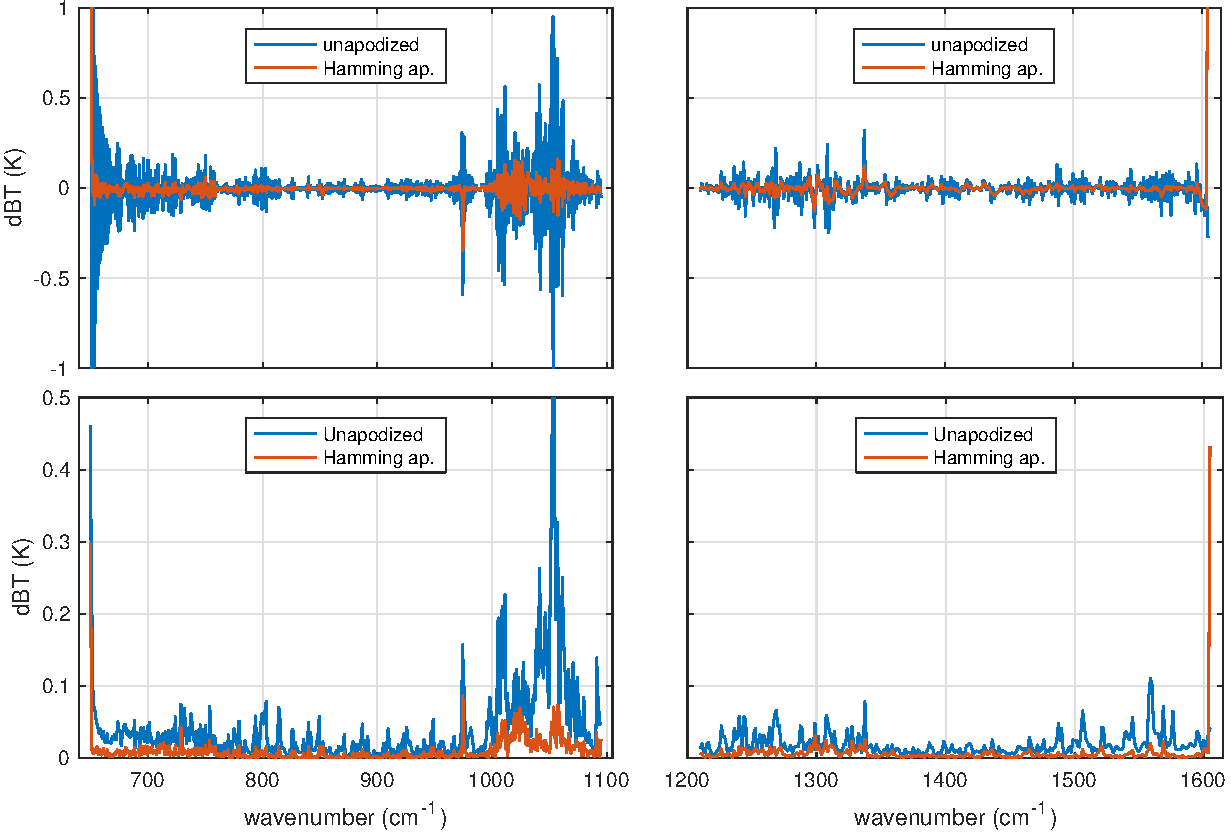
\includegraphics[width=\linewidth]{./figs/airs2cris_validation_LW_MW.pdf}
\caption{
  Brightness temperature spectra for AIRS to CrIS LW band.}
\label{fig:1a}
\end{figure}

%\begin{figure}[htb]
%\centering
%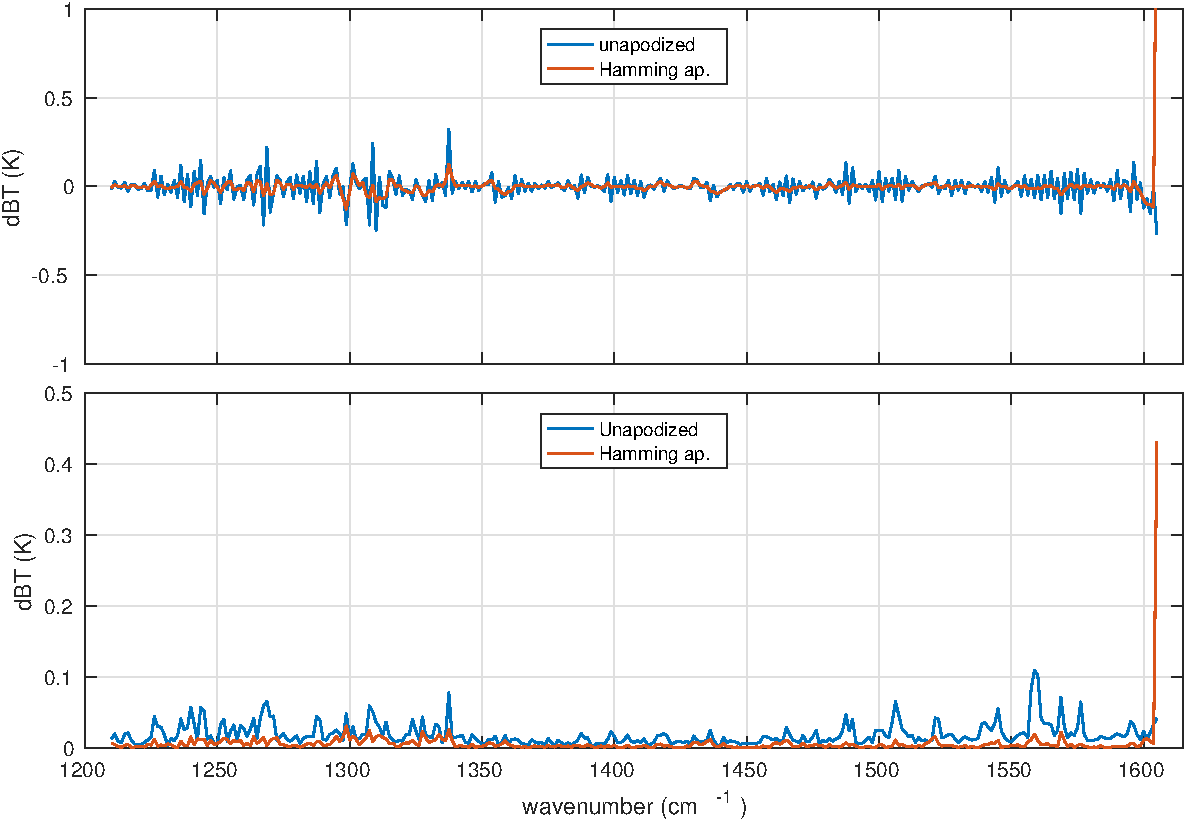
\includegraphics[width=\linewidth]{./figs/airs2cris_vs_truth_MW.pdf}
%\caption{
%  Brightness temperature spectra for AIRS to CrIS MW band.}
%\label{fig:1b}
%\end{figure}

Validation of the IASI to CrIS deconvolution using the 49 test profiles and kcarta simulations are shown for the LW and MW bands of CrIS in figure \ref{fig:2a}. Points to note include: 1). There is no mean bias trend across the band 2). The mean residuals and standard deviation are not significant and < 0.1 mK across the band, except for the few channels at band edges.

\begin{figure}[htb]
\centering
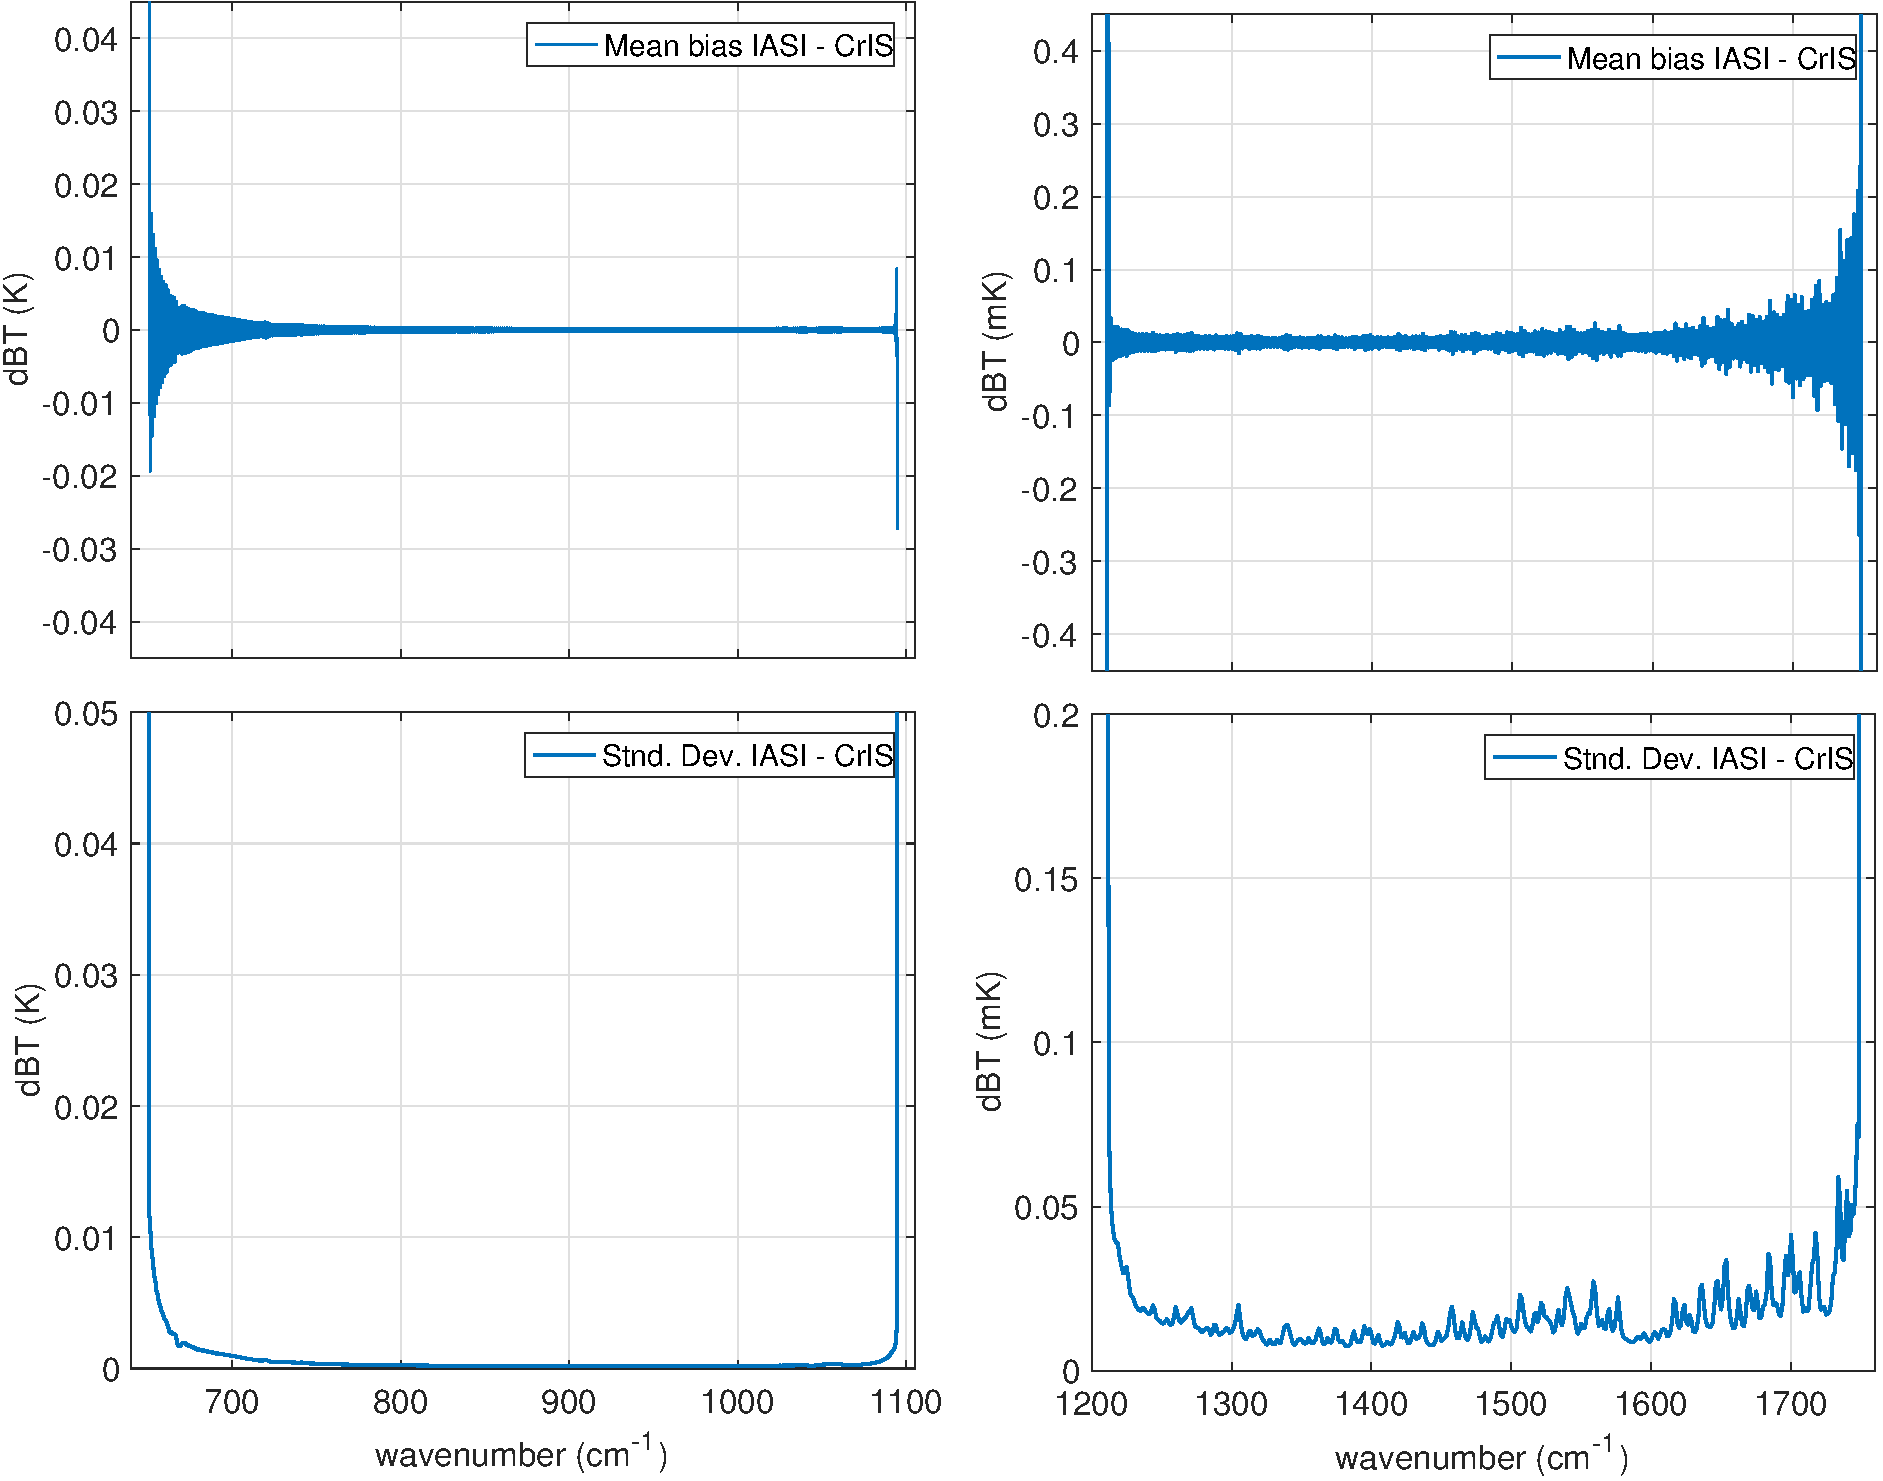
\includegraphics[width=\linewidth]{./figs/iasi2cris_validation_LW_MW.pdf}
\caption{
  Brightness temperature spectra for IASI to CrIS LW (left) MW (right) band. Note the change of y-scale}
\label{fig:2a}
\end{figure}

%\begin{figure}[htb]
%\centering
%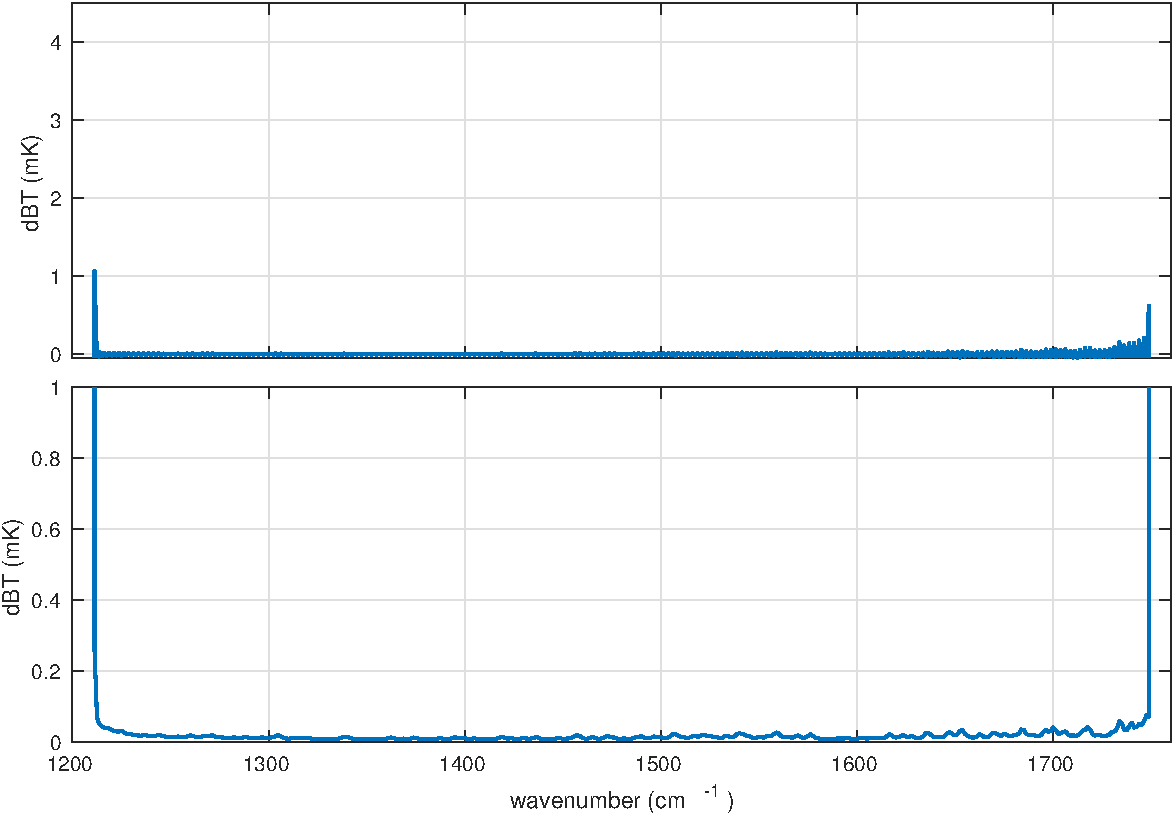
\includegraphics[width=\linewidth]{./figs/iasi2cris_vs_truth_MW.pdf}
%\caption{
%  Brightness temperature spectra for IASI to CrIS MW band. Note the milli-Kelvin scale.}
%\label{fig:2b}
%\end{figure}


\section{Results}
The following sub-sections summarize the bias between each pair of sensors as a function of wavenumber for the selected SNO samples. For the IASI:CrIS and AIRS:CrIS SNOs, the IASI and AIRS spectral radiances are converted to the CrIS grid.  For the AIRS:IASI SNOs, the IASI are converted to the AIRS grid. Lastly, a summary for the double difference of AIRS and IASI compared to CrIS is given. We propose using the common radiance record on the CrIS spectral channels for the climate radiance record. Some discussion and methods to account for biases between the different sensors are provided. In this study, for brevity, we do not consider the shortest wavelength channels that are affected by reflected solar radiation.

\subsection{IASI and CrIS SNOs}
The selection criteria for the IASI and CrIS SNOs are that any of the prescribed fields of view (FOV) (see above) between each sensor are less than 13 km and 20 minutes apart. This choice trades minimizing the effect of non-uniform scenes and retaining large numbers of samples.  For each SNO pairing the FOVs are recorded. The data encompass the period from April 2012 to February 2014, in which there are 275,511 SNO pairs. Because of the different orbits
of Suomi-NPP and Metop-A the coincident observations only occur at high latitudes as
shown in figure \ref{fig:X1}

\begin{figure}[htb]
\centering
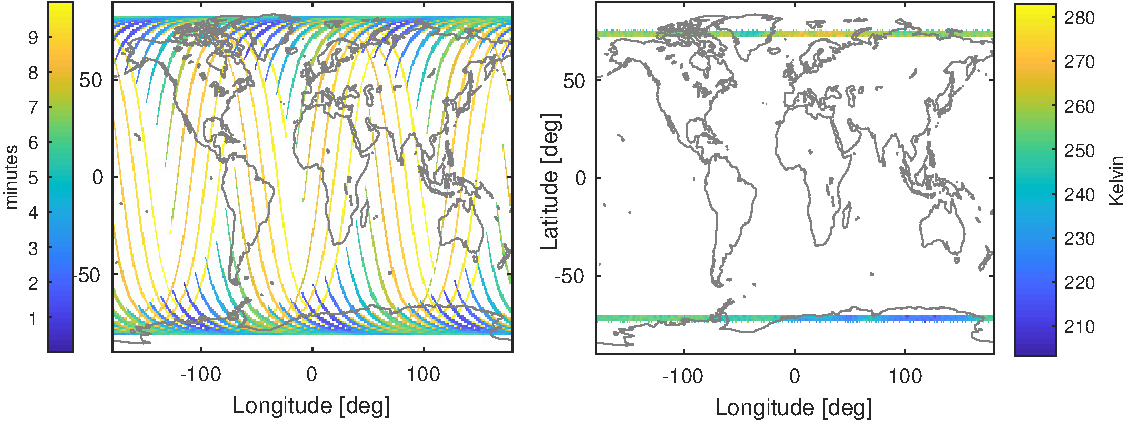
\includegraphics[width=\linewidth]{./figs/AC_IC_jplSNO_maps.pdf}
\caption{
  SNO Location maps. Left: AIRS:CrIS showing time delay. Right: IASI:CrIS, showing $900 cm^{-1}$ brightness temperature.}
\label{fig:X1}
\end{figure}

Note that because the latitude range is very restricted, the dynamic range will be limited and rather low; the warmest scenes will be clear views of the Norwegian Sea in boreal summer.  Furthermore, there will tend to be high sensitivity to scene inhomogeneity in the window channels, with land/sea ice and ocean contrasts in close proximity. For example, the population of
the brightness temperatures for the set in the 900 $cm^{-1}$ window channel is shown in figure \ref{fig:X2}. Notice how similar are the distributions of the two sensors.
The observed brightness temperature range in the window is from about 190 K to 300 K. Clearly,
the majority of scenes involve ice, in the form of cloud or on the ground or ocean.

\begin{figure}[htb]
\centering
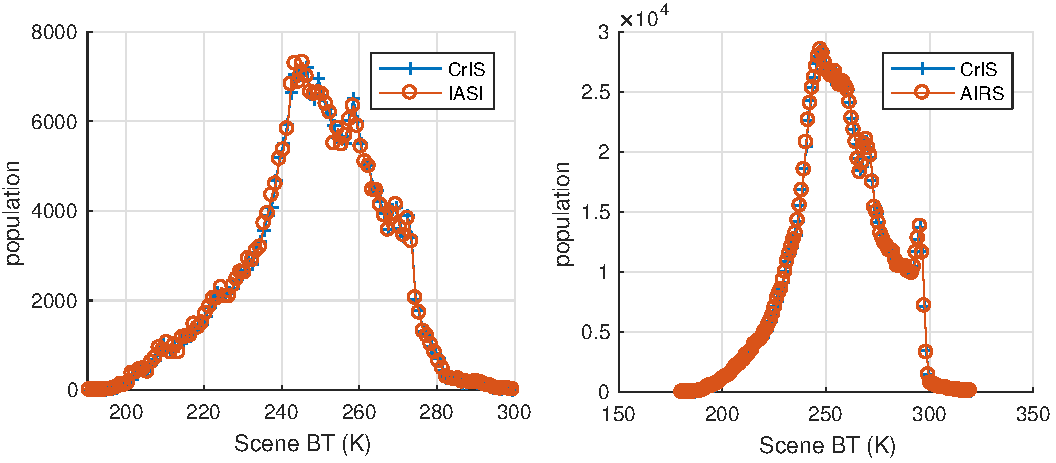
\includegraphics[width=\linewidth]{./figs/AC_IC_jplSNO_900wn_hist.pdf}
\caption{
  SNO PDFs. Left: CrIS:IASI $900 cm^{-1}$ channel. Right: AIRS:CrIS $900 cm^{-1}$ brightness temperature distribution vs scene bin.}
\label{fig:X2}
\end{figure}

Evaluation of the bias between the two sensors is achieved by first converting all the
IASI spectra on to the CrIS spectral grid, using the deconvolution tool described above.
In figure \ref{fig:X3} the average difference of all SNO pairs
is evaluated, together with the standard error of the mean difference. A very few
observations are eliminated based on the quality flag available in the L1C file, and some other non-physical observations are elimited based on extreme 6-sigma outliers. This generally removes less than  0.1\%  of samples. Notice the general slope in bias from 0.2 K to about 0.5 K from the long-wave to short wave end. The large bias of the first two or three channels at the ends of this band reflect the band edge limit of the deconvolution, and are not used.

\begin{figure}[htb]
  \centering
  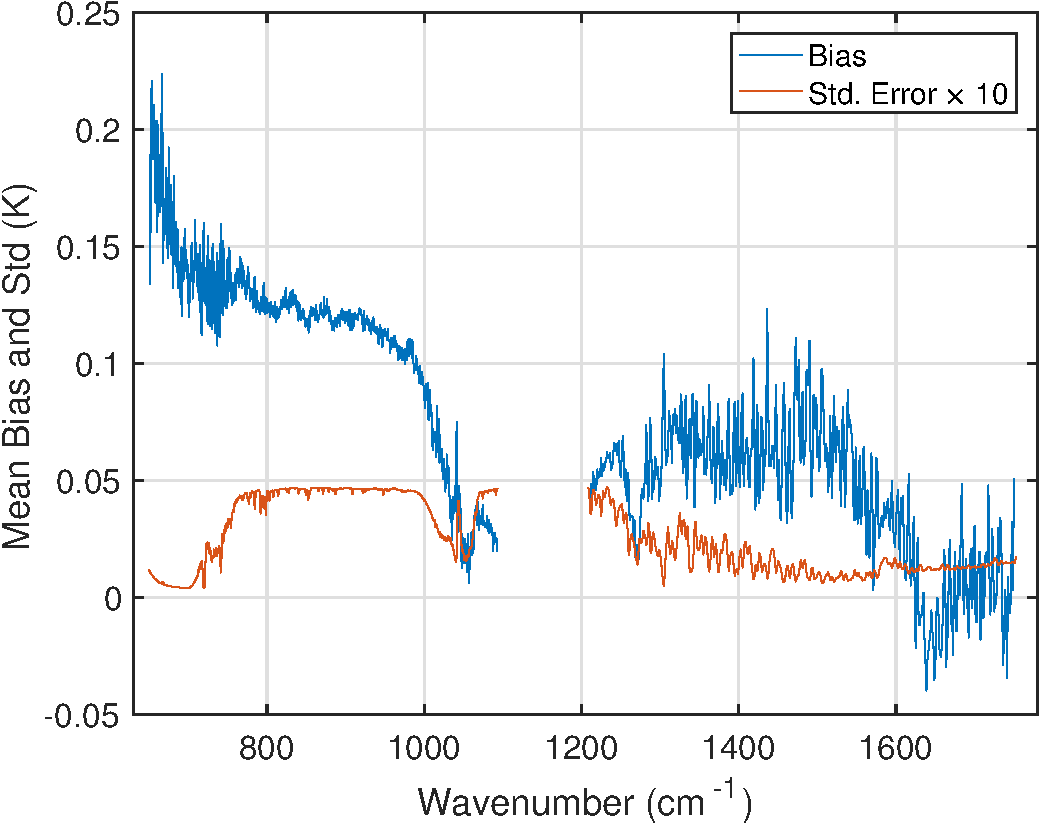
\includegraphics[width=\linewidth]{./figs/fig5_singlecolumn.pdf} 
  \caption{CrIS - IASI bias (K) for all SNO samples from the set.}
  \label{fig:X3}
\end{figure}

There are many different ways to examine more closely the characteristics of the bias with this data set. Here, the sample is subset based on whether the scenes are in day-time (sun-lit) or night-time (eclipsed), and on whether they are in the north or south polar regions. This also provides a convenient warm and cold subset. Figure \ref{fig:X5} shows the mean spectra and the mean bias and standard error of the mean bias between IASI and CrIS for the day/night subsets. Notice, that despite the
relatively large difference in the mean brightness temperatures between the two subsets, the biases are very similar.

%\begin{figure}[htb]
%\centering
%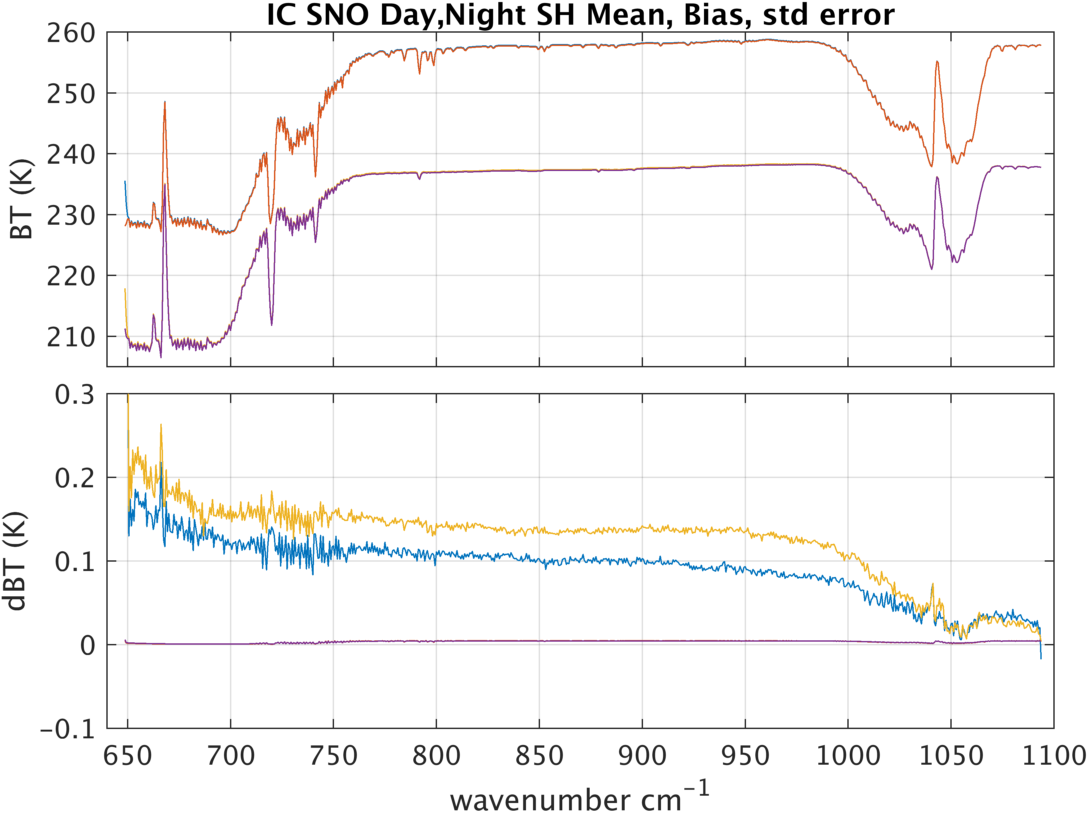
\includegraphics[width=\linewidth]{./figs/IC_jplSNO_dayNight_Bias_stdErr_LW.png}
%\caption{
%  CrIS - IASI bias (K) subset by day and night. Upper panel shows the mean brightness temperature %spectrum. Lower panel the mean bias and standard error of the bias for each of the day/night %subsets.}
%\label{fig:X5}
%\end{figure}

%\begin{figure}[htb]
%\centering
%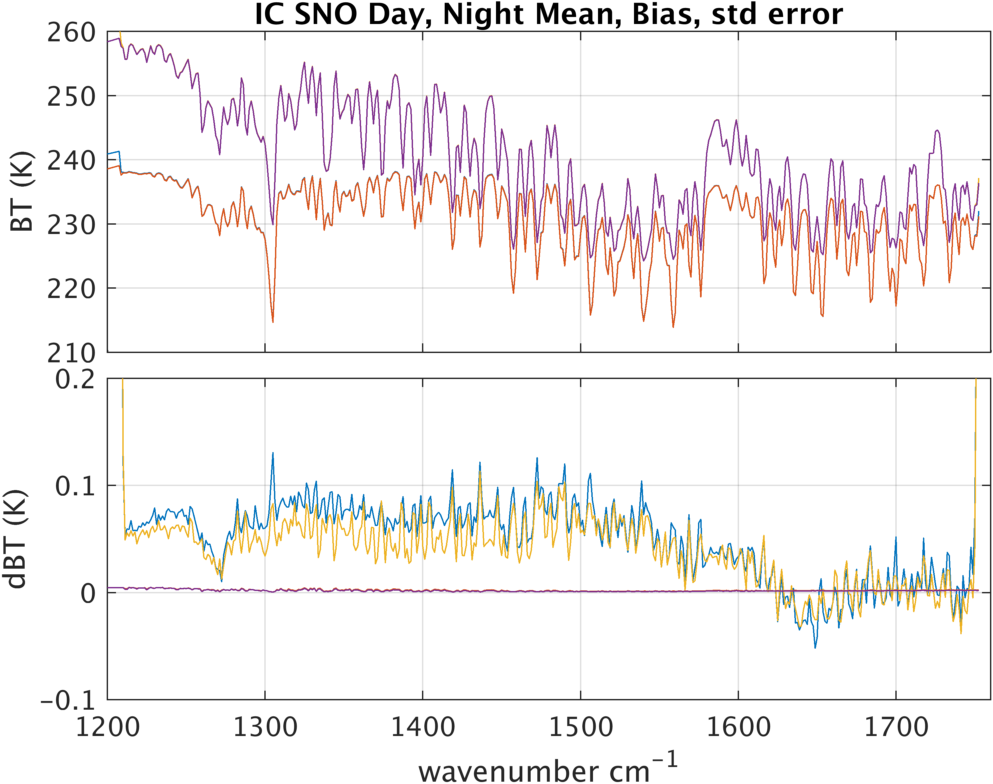
\includegraphics[width=\linewidth]{./figs/IC_jplSNO_DayNight_Bias_stdErr_MW.png}
%\caption{
%  CrIS - IASI bias (K) subset by day and night. Upper panel shows the mean brightness temperature %spectrum. Lower panel the mean bias and standard error of the bias for each of the day/night %subsets.}
%\label{fig:X6}
%\end{figure}


\begin{figure*}[htb]
    \centering
    \subfloat[Long Wave]
             {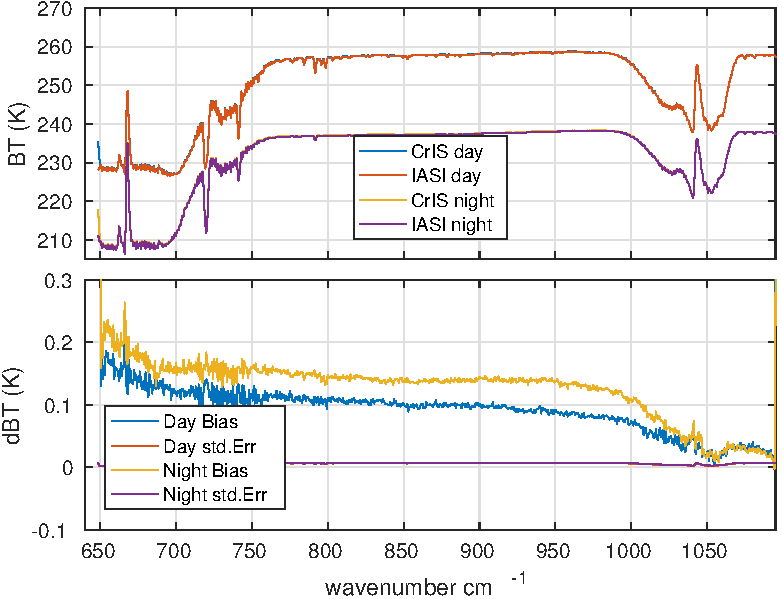
\includegraphics[width=0.48\linewidth]{./figs/IC_jplSNO_dayNight_Bias_stdErr_LW.pdf} }
    \subfloat[Medium Wave]
{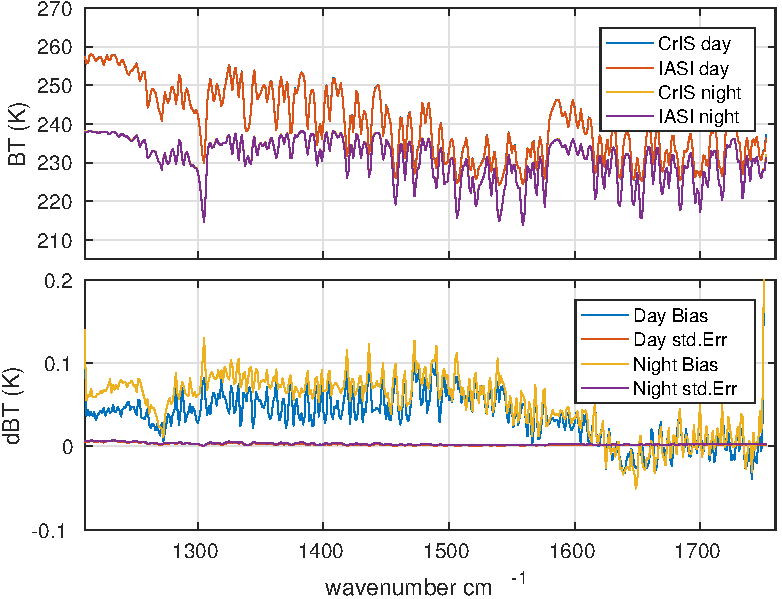
\includegraphics[width=0.48\linewidth]{./figs/IC_jplSNO_dayNight_Bias_stdErr_MW.pdf} }
    \caption{CrIS - IASI bias (K) subset by day or night. Upper panel: Mean brightness temperature. Lower panel: mean bias and standard error.}
    \label{fig:X5}
\end{figure*}

Figure \ref{fig:X7} shows the mean spectra, the mean bias and the standard error of the bias for the north and south subsets.
As with the day/night subset although the scenes are very different the mean biases are
very similar.

\begin{figure*}[htb]
  \centering
  \subfloat[Long Wave]
           {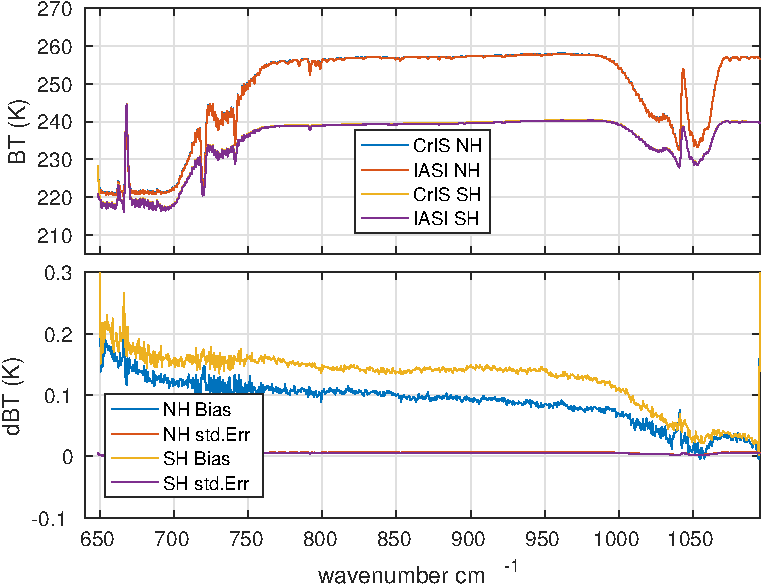
\includegraphics[width=0.48\linewidth]{./figs/IC_jplSNO_northSouth_Bias_stdErr_LW.pdf}}
\hfill
  \subfloat[Medium Wave]
           {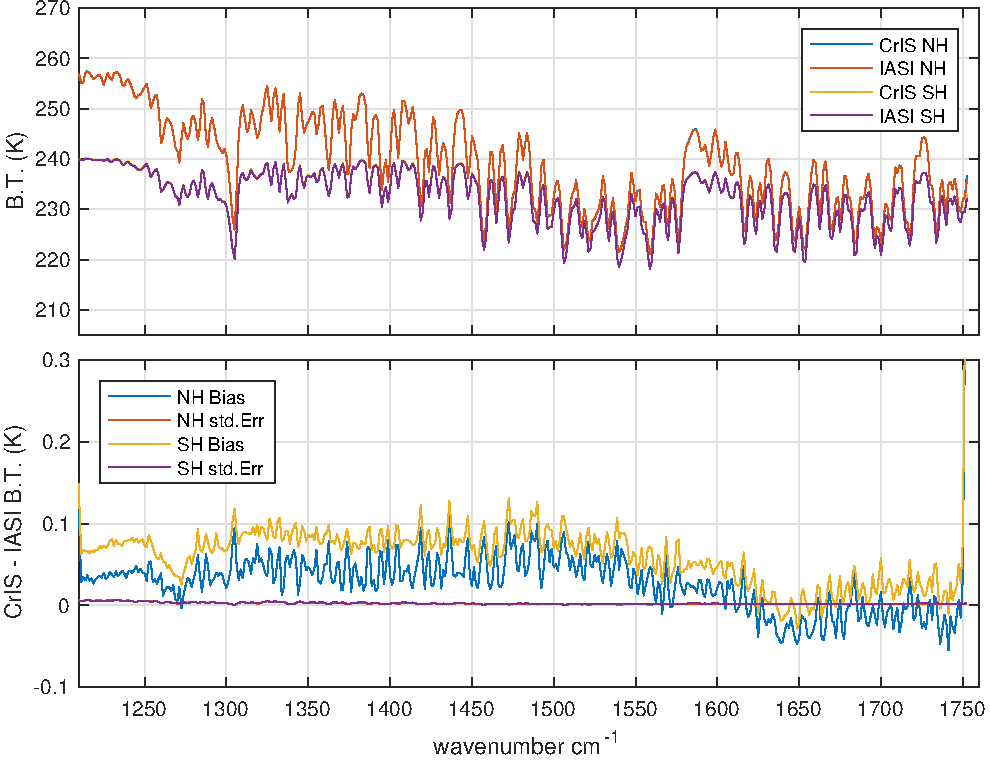
\includegraphics[width=0.48\linewidth]{./figs/IC_jplSNO_northSouth_Bias_stdErr_MW.pdf}}
  \caption{CrIS - IASI bias (K) subset by north or south hemisphere. Upper panel: Mean brightness temperature. Lower panel: mean bias and standard error.}
  \label{fig:X7}
\end{figure*}

To determine if the bias varies over the brightness temperature of the scenes, the SNO pairs are binned according to the BT for each channel from each pair. The contribution from each sensor in each BT bin is included without duplication.  A fine-grained quantile profiler is used to select the bin values for each channel, since different wavelengths will see different dynamic ranges.  In dividing up the samples into small bins it will be noticed that at the hot and cold ends of the range some bins have too few samples to be useful, as can be seen from figure \ref{fig:X8}, in which the standard error grows very large. This figure shows the result both for a single channel at $900 cm^{-1}$ and the the mean bias of 160 window channels from about $800\ to\ 900 cm^{-1}$. Note that in this plot the bias is the CrIS minus IASI bias observation. Examining this figure suggests that the bias is rather close to zero near 270 K, and increases slightly to colder scenes, with CrIS observations warmer than IASI. Also that the bias variation with scene
is very consistent amongst all these channels. Due to the sample size in the bins used here, the valid range is from about 210 K to 280 K scenes, outside this range the estimate of bias is unreliable.
At this point it would be speculation to attribute the variation of bias as a function of radiance, as it could be due to non-linearity of either or both sensors, for example. This study of scene dependent bias can be extended to all channels (not shown here).

%\begin{figure}[htb]
%\centering
%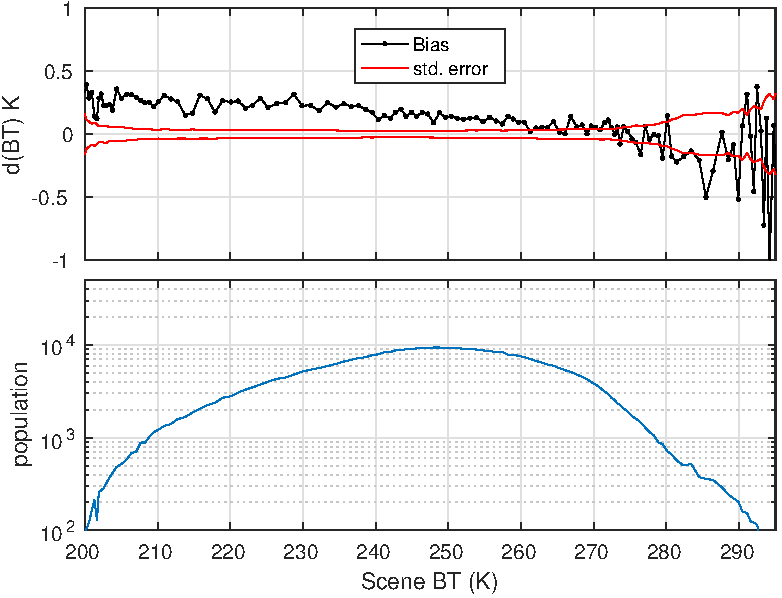
\includegraphics[width=\linewidth]{./figs/IC_jplSNO_Bias_stdErr_900wn_vsScene_quantile.pdf}
%\caption{
%  CrIS-IASI bias (K) for channel at $900 cm^{-1}$ as a function of scene brightness temperature, %upper panel, together with the standard error. Lower panel shows the sample size in the bins.}
%\label{fig:X7}
%\end{figure}

%Taking 160 window channels from about $800\ to\ 900 cm^{-1}$, the bias variation with scene
%is very consistent amongst these channels, summarizing these in figure \ref{fig:X8} showing the %mean bias and standard deviation of the bias. Taking small groups of channels starting at the %longest wavelength (lowest numbered) shows the the bias is more constant with scene temperature %and from about 710 $cm^{-1}$ the bias takes on a slope like that shown in figure \ref{fig:X7}. At %this point it would be speculation to attribute the variation of bias as a function of radiance, %as it could be due to non-linearity of either or both sensors, for example. This study of scene %dependent bias can be extended to all channels (not shown here).

\begin{figure}[htb]
\centering
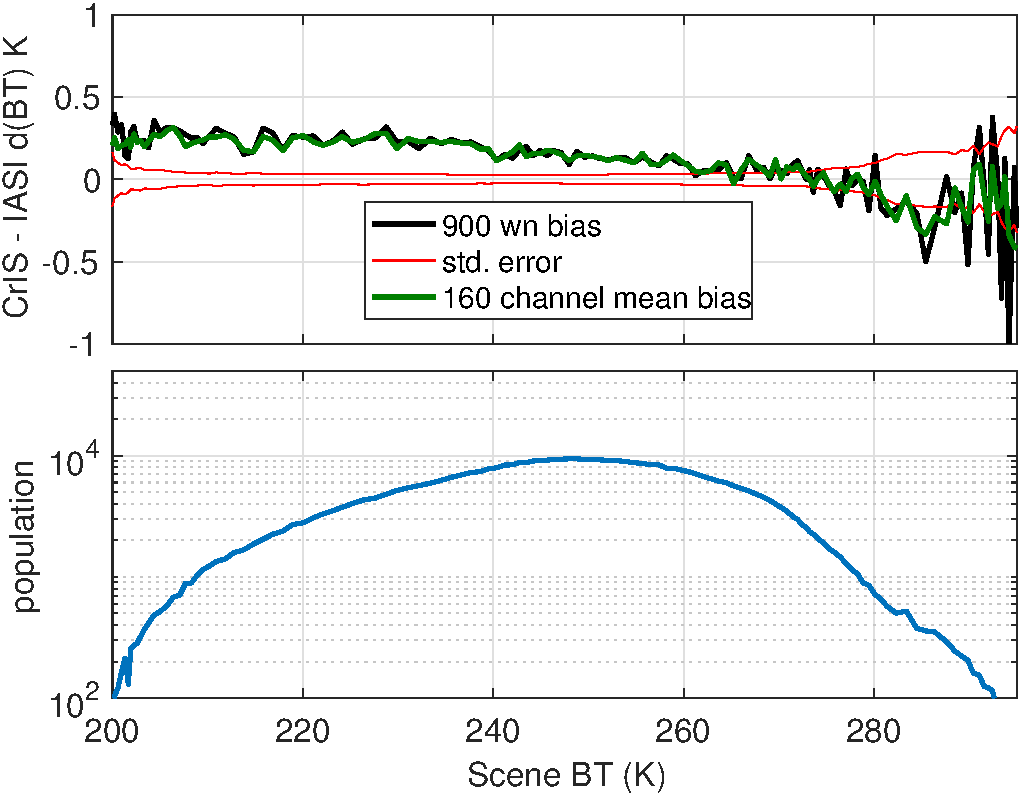
\includegraphics[width=\linewidth]{./figs/ic_jpl_sno_bias_stderr_vs_scene_LW_chans.pdf}
\caption{
  CrIS-IASI bias (K) for a single channel at 900 cm$^{-1}$ and mean bias of 160 channels from 800 to 900 cm$^{-1}$ as a function of scene brightness temperature together with the standard deviation. Lower panel shows the opulation size per temperature bin.}
\label{fig:X8}
\end{figure}


\subsection{AIRS and CrIS SNOs}

The selection criteria of the AIRS and CrIS SNOs (see above) are that the FOVs are located
within 13 km and within 10 minutes of each other. For each SNO pair the CrIS FOV is recorded. 

The data set encompasses the calendar year 2013. There are $1.393\times 10^{6}$ pairs, and they are distributed as shown in figure \ref{fig:X1}.

%For the tropical v10.0.0 set there are 4.232 x10$^{\text{6}}$ SNO pairs, distributed within 50 degrees latitude of the equator. For the 'standard' JPL set . 
Note i) there is a much higher surface-area density of data near the poles; 
ii) Nearer the equator all pairs have a positive time delay, greatest at the equator with AIRS later than CrIS. The ascending node is at 1:30 pm, with
AIRS samples later after local solar noon than the CrIS samples during the day; 
iii) Only descending orbit (night) samples are available over Africa and Australia and only day time ones over South America, this has significant impact on the hot bias of the samples. Also note that even with close spatio-temporal sampling, the estimate of bias between the sensors will be better where the scene is more uniform.

%\begin{figure}[htb]
%\centering
%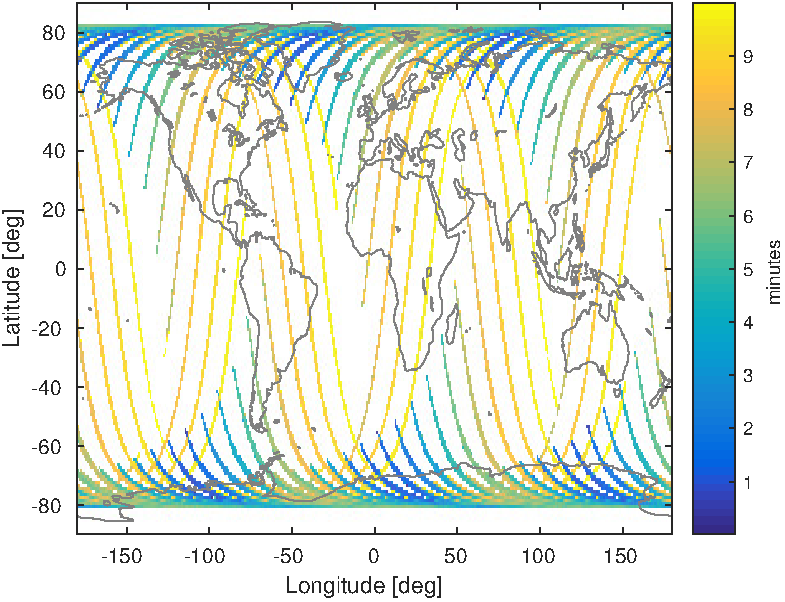
\includegraphics[width=\linewidth]{./figs/AC_jplSNO_delay_map.pdf}
%\caption{
%  Global distribution of the AIRS, CrIS SNO set. Color indicates delay time in minutes.}
%\label{fig:Y1}
%\end{figure}

Notice that the brightnes temperature distribution for the window channel at $900 cm^{-1}$ is highly non-Gaussian, with a sharp drop and short hot tail and longer cold tail, indicative of large numbers of warm ocean samples, and a variety of clouds, respectively, as shown in figure \ref{fig:X2}. In particular note that: 
ii) The hottest scenes, greater than about 303 are exclusively over land during the day, with a very few up to 331 K; 
iii) the peak around 295 K is indicative of clear tropical ocean scenes; 
iv) the peak around 270 K is probably freezing water; 
v) the relatively large population from about 240 K to 260 K is due to the large number of cold polar scenes and cold clouds. The fact that most samples with zero time delay occur exclusively at high latitudes and all tropical samples have the largest time delays has important consequences on how to interpret biases for these samples.

For channels that are at wavelengths with weighting functions that peak higher in the atmosphere, the distributions tend to be more Gaussian than the window channels, with brightness temperatures populations that peak at levels dependent upon the altitude of the weighting function. In general the window channels provide the largest BT dynamic range.

%\begin{figure}[htb]
%\centering
%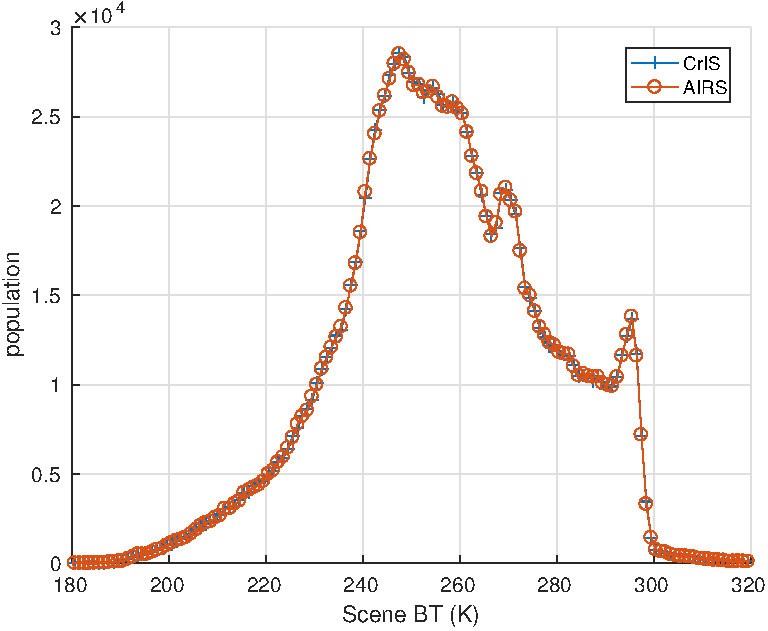
\includegraphics[width=\linewidth]{./figs/AC_jplSNO_900wn_population_vs_scene.pdf}
%\caption{
%  Population distribution for the $900 cm^{-1}$ window channel as function of scene.}
%\label{fig:Y2}
%\end{figure}

%\begin{figure}[htb]
%\centering
%\includegraphics[width=.9\linewidth]{../../gitLib/asl_sno/run/figs/2013_AC_trop_Airs_900wn_hist.pdf%}
%\caption{
%Population distribution of JPL Tropical 2013 subset.}
%\end{figure}

%\begin{figure}[htb]
%\centering
%\includegraphics[width=.9\linewidth]{../../gitLib/asl_sno/run/figs/2013_AirsCris_jpl_tropStnd_delay%Hist.pdf}
%\caption{
%Sensor sample delay (Airs observation time - CrIS observation time).}
%\end{figure}

%For example, figure \ref{fig:Y5} is a plot of an average spectrum 
%of AIRS and CrIS for a sample of the SNO data. Notice that on this plot the AIRS data are level 1b, %and contain some un-filtered bad channels that are not used in the final
%bias calculations. 
%\begin{figure}[htb]
%\centering
%\includegraphics[width=.9\linewidth]{../../gitLib/asl_sno/run/figs/2013_trop_Airs_CrIS_Sample_Average_%Spectrum.pdf}
%\caption{
%Sample brightness temperature spectrum from the SNO set (Airs blue).}
%\end{figure}

With the conversion of AIRS level 1b radiance spectra first to the clean and filled level 1c
then to the CrIS spectra grid, allows bias differences to be evaluated for the
channels that are common to both AIRS and CrIS. An example of the mean brightness
temperature bias CrIS-AIRS for the long wave (LW) band for all SNO samples in this
data set, is shown in figure \ref{fig:Y6}. Notice that the standard error is very small.

\begin{figure*}[htb]
  \centering
  \subfloat[Long Wave]{
     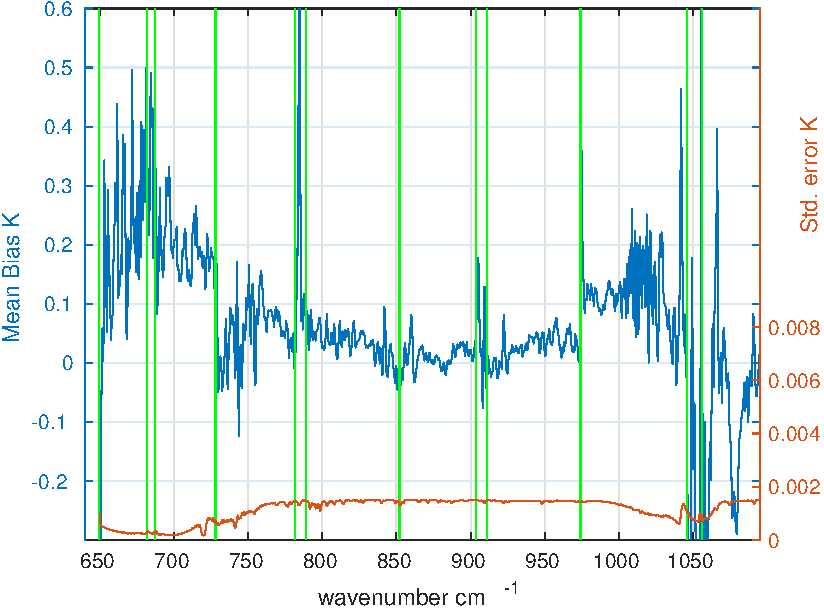
\includegraphics[width=0.48\linewidth]{./figs/AC_jplSNO_Bias_stdErr_wModEdges_LW.pdf}}
  \subfloat[Medium Wave]{
     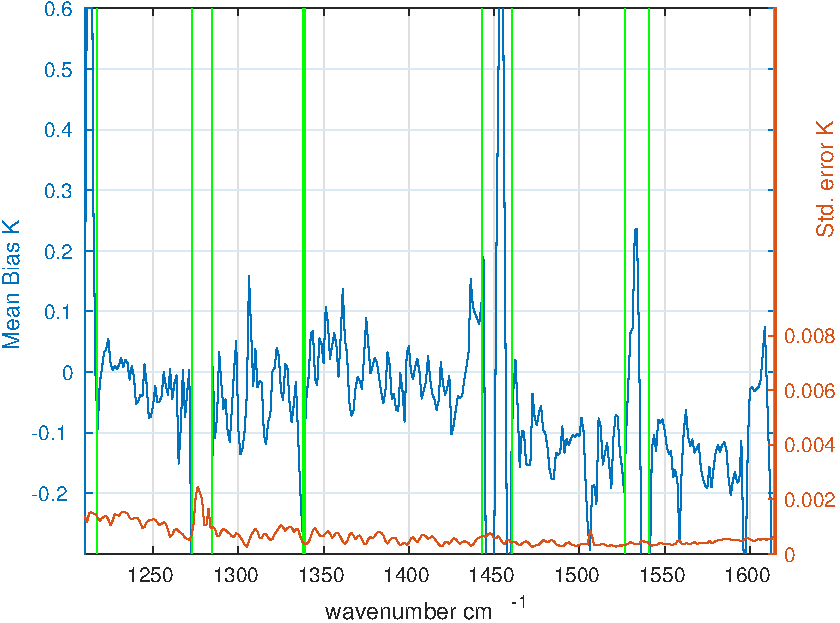
\includegraphics[width=0.48\linewidth]{./figs/AC_jplSNO_Bias_stdErr_wModEdges_MW.pdf}}
  \caption{
    CrIS - AIRS mean bias and standard error of the SNO set. Vertical bars mark AIRS array module boundaries.}
  \label{fig:Y6}
\end{figure*}

%\begin{figure}[htb]
%\centering
%\includegraphics[width=.9\linewidth]{../../gitLib/asl_sno/run/figs/2013_AC_jplSNO_std_LW_biasSte_wModu%les.pdf}
%\caption{
%2013 Tropical SNO mean sample bias (AIRS - CrIS) in the LW band.}
%\end{figure}

%\begin{figure}[htb]
%\centering
%\includegraphics[width=.9\linewidth]{../../gitLib/asl_sno/run/figs/2013_AC_jplSNO_std_MW_biasSte.pdf}
%\caption{
%2013 standard SNO mean sample bias (AIRS - CrIS) in the MW band.}
%\end{figure}

Note that the original AIRS spectrum of observations include the repaired bad channels and filled gaps, before the spectrum is converted to the CrIS grid, therefore those artifacts are carried through to these spectral biases. In the final analysis only the original AIRS L1b channels that passed the quality screening used in the L1C processor are selected for evaluation of bias. Figure \ref{fig:Y6} also shows the frequencies of the AIRS array module edges. One can see the effect of different gain settings for some of the different modules as well as edge effects. In addition, several small spectral regions do not have any AIRS detectors and so a reconstructed during the AIRS L1C processing. These show up in the bias plots, for example $ 682 - 688 cm^{-1} $, $ 782 - 790 cm^{-1} $, $ 904 - 911 cm^{-1} $, $ 1046 - 1056 cm^{-1} $, $ 1272 - 1284 cm^{-1} $, $ 1443 - 1460 cm^{-1} $, $ 1527 - 1541 cm^{-1} $.

The division of the AIRS:CrIS SNOs into day/night or north/south hemisphere subsets does not reveal a significant separation of bias and are not shown here.

The variation of bias between AIRS and CrIS with scene brightness temperature is shown in figure \ref{fig:Y7} for a channel at $ 900 cm^{-1} $. As with the IASI:CrIS comparison the bias is not constant over the dynamic range of interest. The estimate of uncertainty using the standard error of the mean bias, shown in this figure, appears to under estimate the true sampling uncertainty where scenes involve extremely hot or extremely cold radiances. The jump in the bias above about 300 K has been investigated in detail and is mostly attributed to scene inhomogeneity. Hot scenes above about 300 K occur exclusively over land during the day and the AIRS observations are always later than the CrIS observations, furthermore, the hottest locations tend to be very localized so there is the added complication of non-uniform scenes and more rapidly changing surface temperatures.

\begin{figure}[htb]
\centering
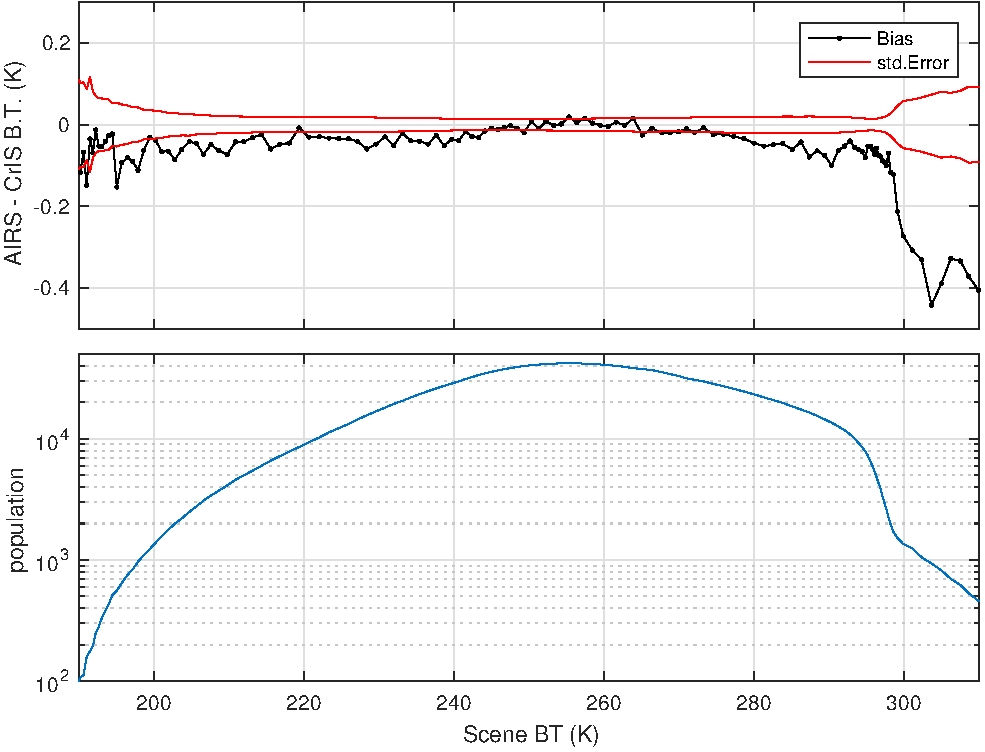
\includegraphics[width=\linewidth]{./figs/AC_jplSNO_900wn_bias_vs_scene.pdf}
\caption{
  SNO data for 2013. Upper: AIRS - CrIS bias for a $900 cm^{-1}$ channel as a function of scene temperature (black line) and the standard error of the mean for the sample (red lines). Lower: Sample size per bin.}
\label{fig:Y7}
\end{figure}

In order to test whether CrIS sees more hot scenes than AIRS the population distribution is determined as a function of scene brightness temperature, for the whole year 2016 and for all fields of view and without restrction to SNO pairing, such that there are no data gaps. The fractional difference in the number of observations is shown in figure \ref{fig:Y8}, and clearly shows that from about 300 K to 320 K there is negligible difference between the two sensors.  

\begin{figure}[htb]
\centering
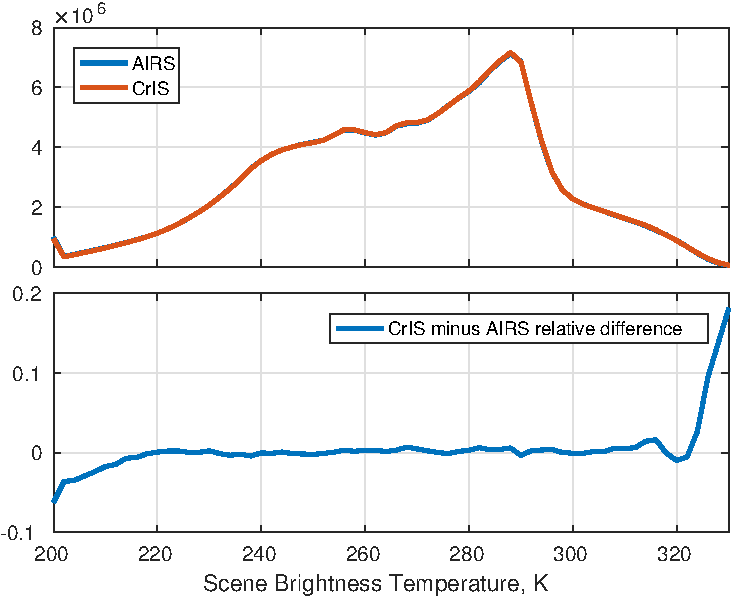
\includegraphics[width=\linewidth]{./figs/full_scan_land_2016_all_mod.pdf}
\caption{
  All observations for 2016, all scan angles, no subsetting. Upper: AIRS and CrIS Observation counts as a function of the $900 cm^{-1}$ channel scene temperature. Lower: fractional difference between the number of AIRS and CrIS in each bin.}
\label{fig:Y8}
\end{figure}

Furthermore, it is known that CrIS uses motion compensation in the scanning mirror so as to remain at a fixed point on the Earth whilst a measurement is obtained. AIRS does not and so it's effective observation footprint will be larger than the geometric FoV as determined by its optical field stops. Since the hot scenes are known by inspection to involve inhomogeneous scenes, the effect can be simulated by taking two adjacent CrIS footprints and taking a weighted average at the SNO observation. Using a $20:80 \% $ average a simulation of the effect of motion smearing can be obtained. Results are shown in figure \ref{fig:Y9}. This clearly shows that the hot bias from about 300 K to 320 K is mitigated. Above about 320 K there are too few samples to be significant and therefor the SNO method for inter-comparison can not be used. The cold scenes are somewhat impacted as expected.

\begin{figure}[htb]
\centering
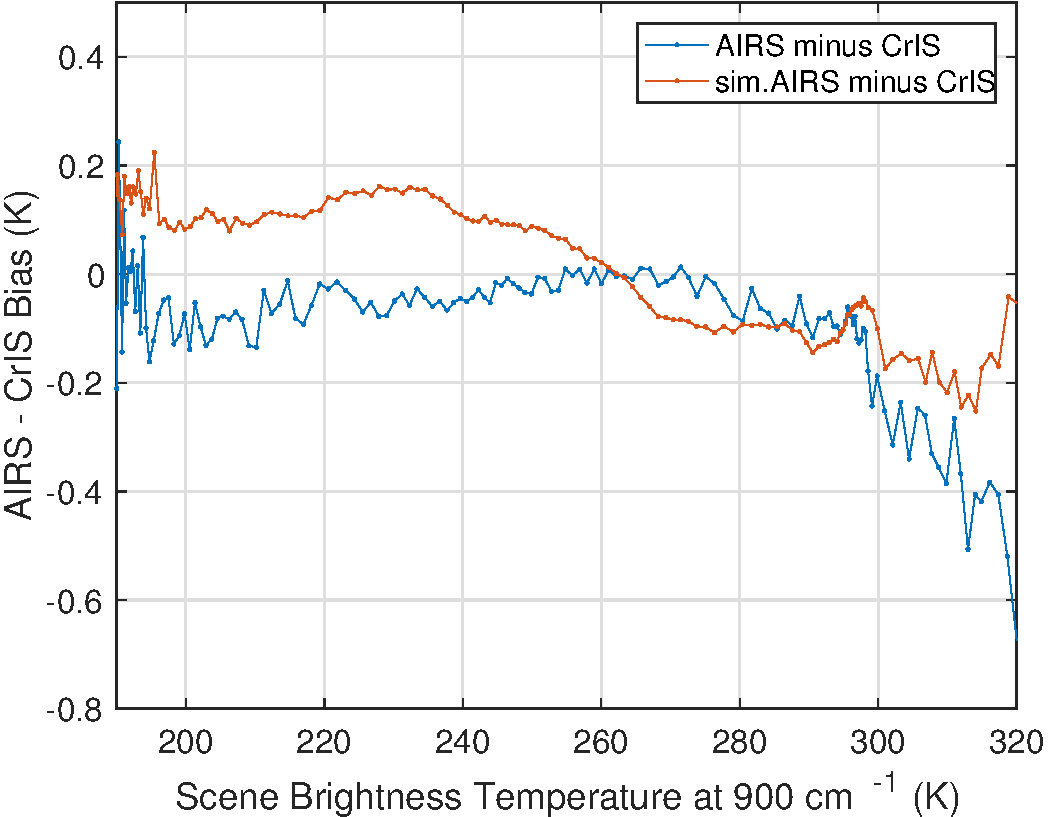
\includegraphics[width=\linewidth]{./figs/2013_ac_quantile_plus_simulated_airs.pdf}
\caption{
  Bias of AIRS minus CrIS for a $900\ cm^{-1}$ channel vs scene B.T. Simulated motion smear compared to original.}
\label{fig:Y9}
\end{figure}

The number of samples in a given month are sufficient to estimate any temporal trend of the bias. This analysis uses an extended SNO data set from summer 2012 to 2015, using CrIS data from the in-house CCAST (CrIS Calibration Algorithm and Sensor Testbed) processing \cite{Motteler2014} and AIRS L1C restricted to tropical scenes. The mean
bias for a 900 $cm^{-1}$ channel for the whole dataset is, within uncertainty, the same as the previous results shown. As before, no spectral drift correction has been applied to the AIRS L1b data to take account of changes in the spectrometer. The trend is estimated to be about 2 to 3 mK per year at 95\% confidence. 

%\begin{figure}[htb]
%\centering
%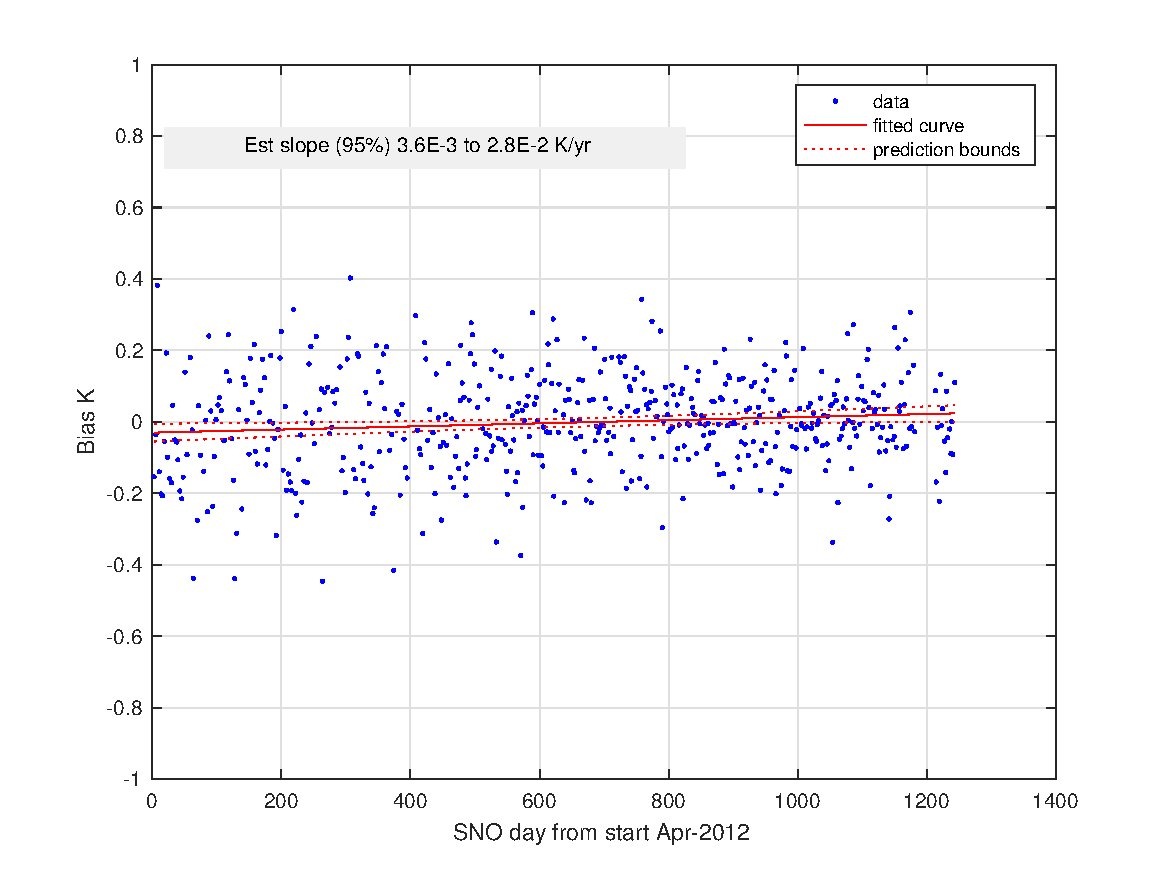
\includegraphics[width=\linewidth]{./figs/AC_aslSNO_900wn_biasTrend_screened.pdf}
%\caption{
%  Temporal bias trend (AIRS - CrIS) for a 900 cm-1 channel}
%\label{fig:Y9}
%\end{figure}


\subsection{AIRS and IASI SNOs}
The AIRS and IASI SNOs are restricted to the near-polar latitudes similar to the 
CrIS and IASI SNOs discussed previously. The criteria for selection based upon spatial and temporal separation is the same as for CrIS and IASI SNOs. The data set used here is for 2013 and consists of about 55,000 SNO pairs. 

The deconvolution of IASI onto the AIRS SRFs will not normally be performed for trending analysis, but is a useful exercise to demonstrate consistency amongst the different sensor pairing. In this study the AIRS L1c data are used therefore the spectral gaps and noisy channels of AIRS have been repaired.
The brightness temperature bias between IASI and AIRS for the LW band using all samples is shown in figure \ref{fig:Z1}, this figure also shows the variation of the bias between AIRS and IASI for the channel at 900 cm${-1}$ as a function of the brightness temperature of the scene. It is possible to conclude that the bias between AIRS and CrIS is less than 0.2 K and over much f the LW band of the order of 0.1 K with a standard error of the mean due to the sampling of about 10 mK.

\begin{figure}[htb]
  \centering
  \subfloat[]{
    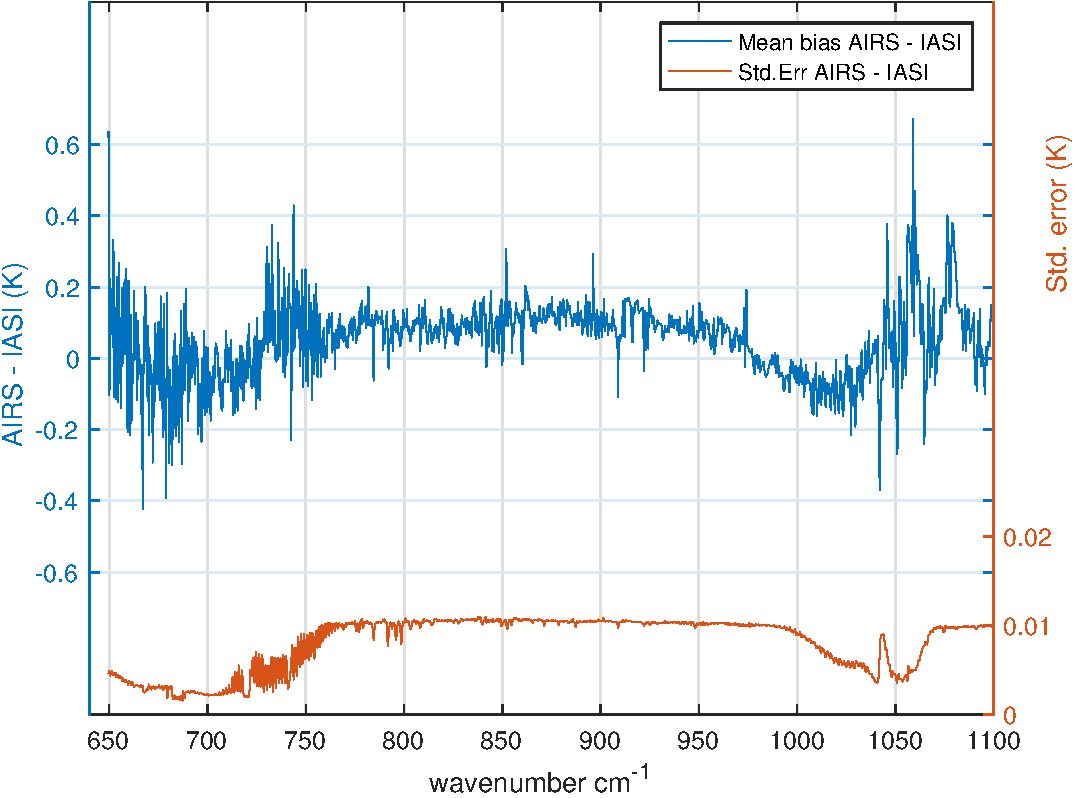
\includegraphics[width=0.48\linewidth]{./figs/2013_ai_l1c_asl_sno_mean_stderr_lw.pdf}}
  \subfloat[]{
    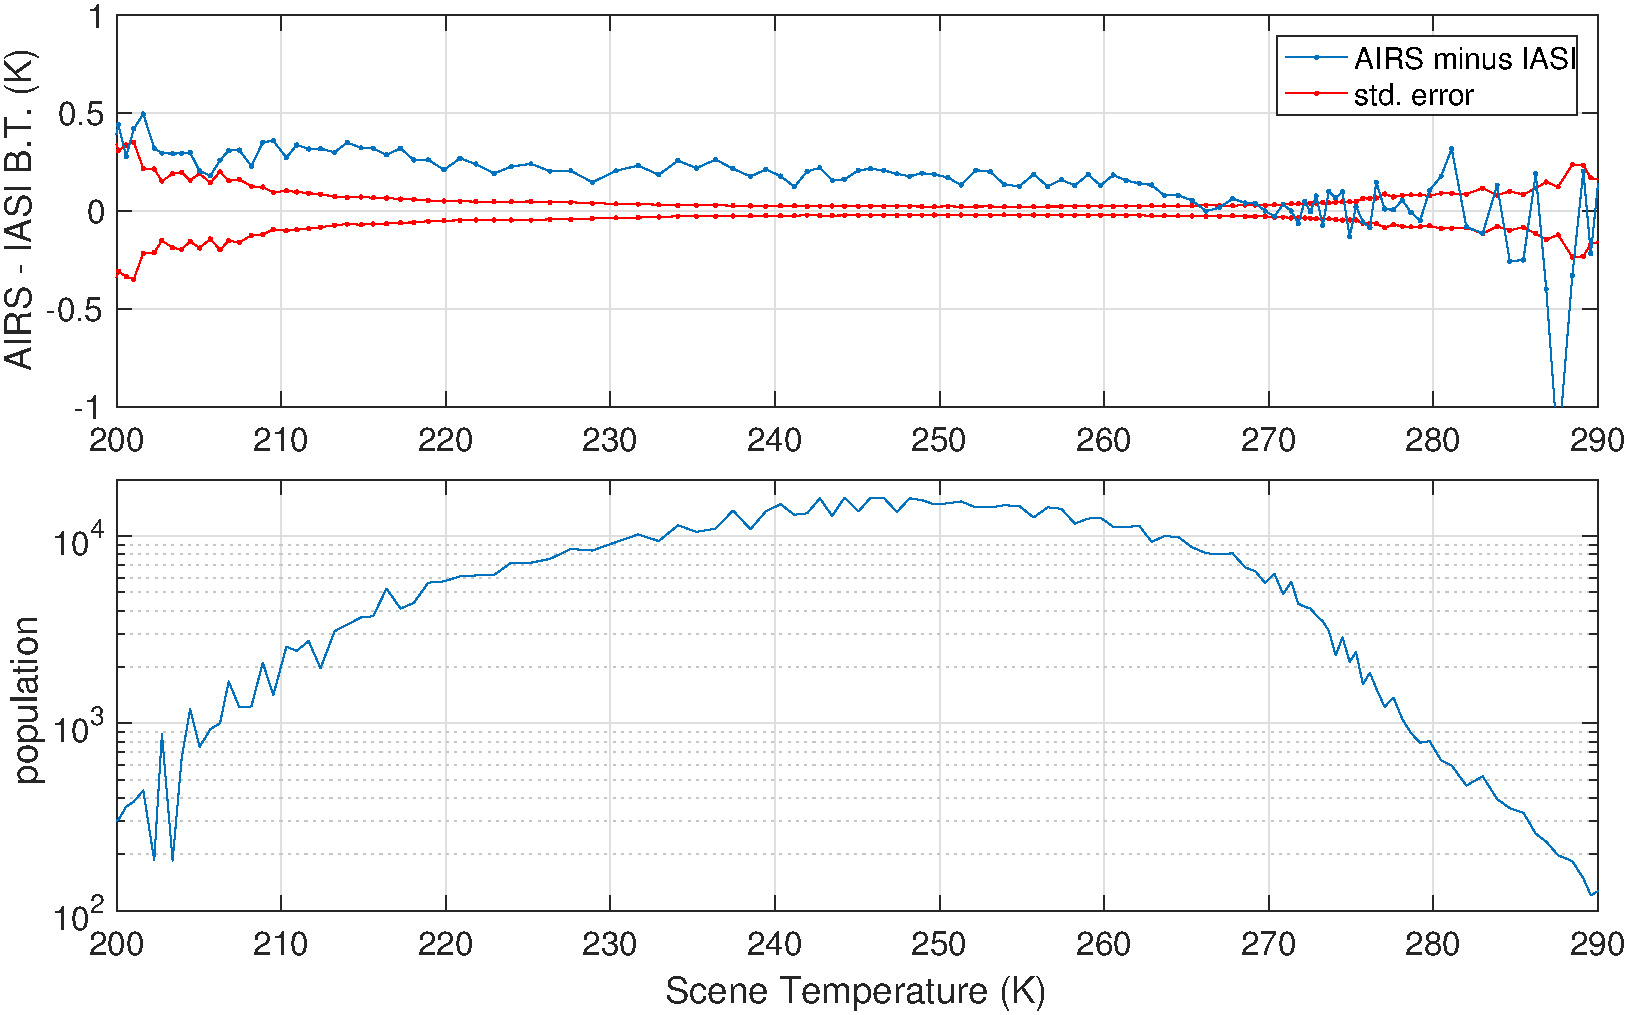
\includegraphics[width=0.48\linewidth]{./figs/AI_jplSNO_bias_std_900wn_vs_scene.pdf}}
\caption{
  2013 AIRS:IASI SNO. a:  mean bias and standard error in the LW band. b: (upper) $900\ cm^{-1}$ channel bias and std. error vs scene B.T. (lower) bin population.}
\label{fig:Z1}
\end{figure}

%For completeness, the variation of bias as a function of scene brightness for the window channel %at $ 900 cm^{-1} $ is shown in figure \ref{fig:Z2}. Notice that most observations are around 250 K %because of the polar coverage.

%\begin{figure}[htb]
%\centering
%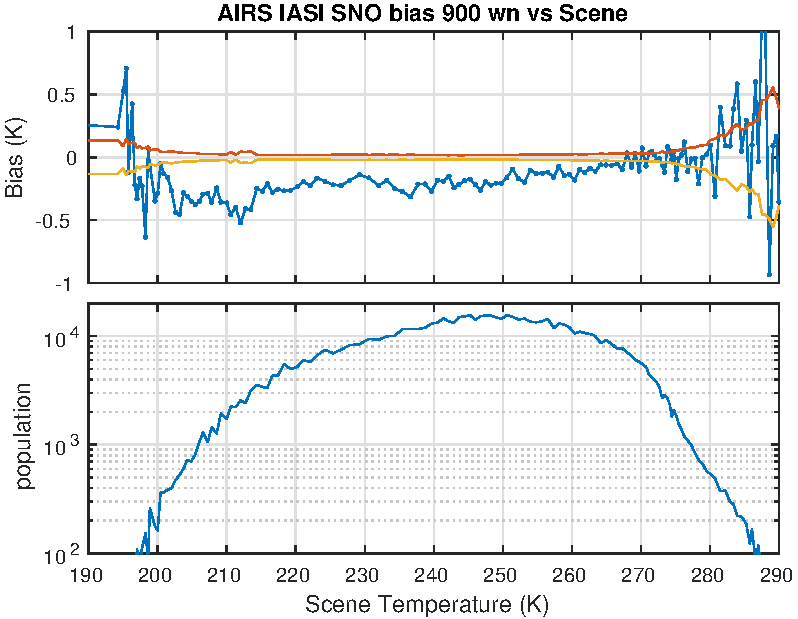
\includegraphics[width=\linewidth]{./figs/AI_jplSNO_bias_std_900wn_vScene.pdf}
%\caption{
%   2013 IASI:AIRS SNO data. Upper: IASI - AIRS bias for the 900 cm window channel as a function of %scene (black line) and the standard error of the mean (red lines). Lower: Sample bin population.}
%\label{fig:Z2}
%\end{figure}



\subsection{AIRS and IASI on the common CrIS grid}
 We can directly compare AIRS, IASI and CrIS using the CrIS response function as the common grid, and choose one of the three as a pseudo-transfer standard for the other two.

The bias for each of the three pairs of sensor SNO sets is shown in figure \ref{fig:U1} for the LW and MW bands. The upper panel shows the AIRS compared to CrIS and IASI and the lower panel CrIS compared to IASI.  The standard errors are not re-plotted here, but have numerical values the same as reported in the preceding sections. Note that in the lower panels, the CrIS - IASI bias follows the double difference of the upper panel.  


\begin{figure*}[htb]
  \centering
  \subfloat[LW]{
    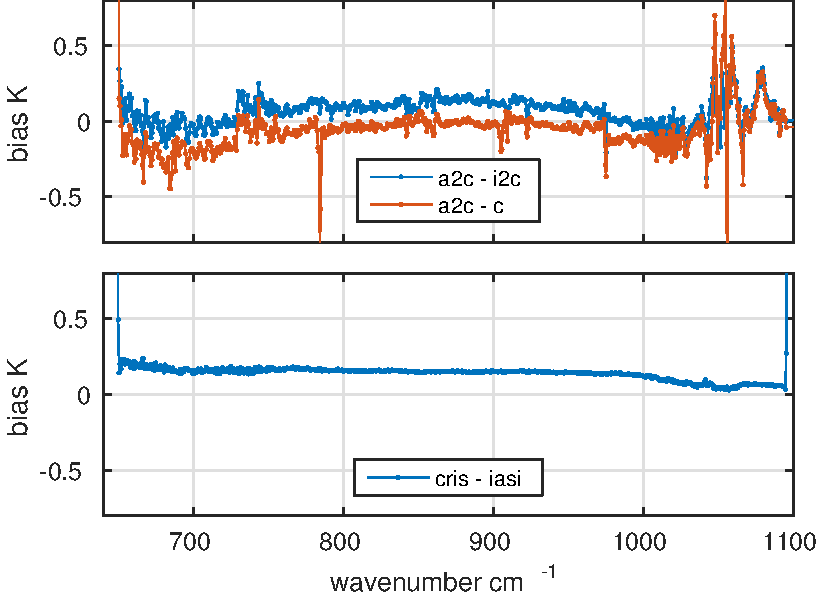
\includegraphics[width=0.48\linewidth]{./figs/AC_AI_CI_biasBT_LW_legend.pdf}}
  \subfloat[MW]{
    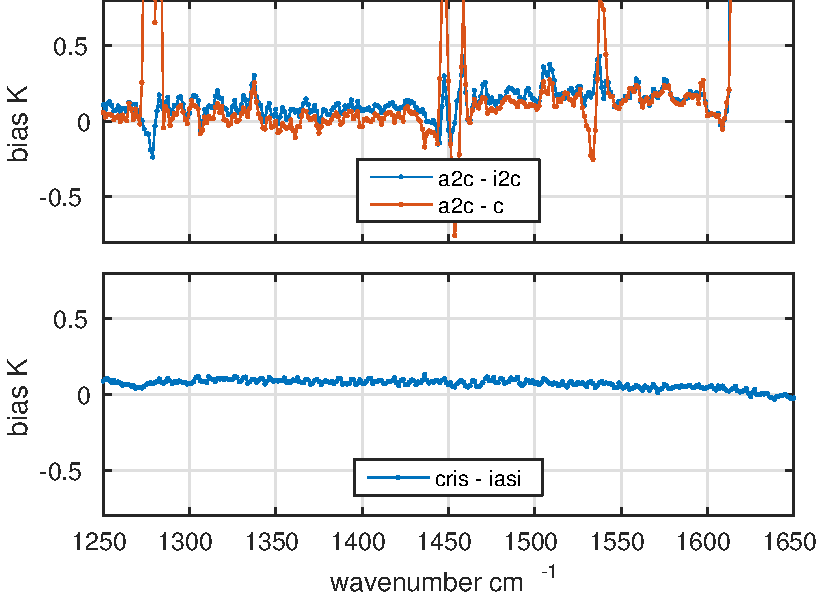
\includegraphics[width=0.48\linewidth]{./figs/AC_AI_CI_biasBT_MW_legend.pdf}}
  \caption{ Combined plot of biases referenced to the CrIS grid. Upper panel: AIRS - IASI (blue) AIRS - CrIS (red), lower panel: CrIS - IASI.}
  \label{fig:U1}
\end{figure*}


\section{Conclusions}
The methods described in this paper provide a quantitative means to determine the bias, expressed in terms of brightness temperature, between different sensors across a relatively large spectral range. It does not, and can not, determine which sensor is the more accurate, but can provide clues as to how a given sensor is behaving when it exhibits the same bias characteristics against two independent sensors. In the case of AIRS, for example, there are distinct changes between some of the different detector modules.

There are a few points to bear in mind when interpreting the results and some limitations of the method, which can be divided into intrinsic and sampling effects. In the deconvolution and translation to a different spectral grid, there tends to be ringing at the boundaries, which is mathematically inevitable, so caution should be made when comparing the first 5 or so channels at the boundaries of the full spectral range. The conversion is perfect where the the spectrum is flat or the nominal resolution perfectly captures the underlying spectral features. Examination of the residuals in the validation plots above, reveal these attributes, however they do not significantly add to the bias. In all cases the conversion to the interferometric ILS spectral wavenumber is followed by Hamming apodization.

In respect of sampling effects, the method would give a perfect analysis of sensor bias if either the Earth scenes were perfectly spatially uniform and static, or the fields of view of the different sensors perfectly matched the same Earth scene at the same time. Furthermore, the results must be interpreted in the context of the dynamic range of the scenes, as illustrated in the figures showing scene dependent bias. Although the sampling is not perfect and scenes not uniform, there are sufficiently large numbers of SNO pairs available that statistical variations can be well characterized and mean bias is statistically significant. This is also illustrated in the scene dependent bias plots. In general, toward the hot and cold extreme scenes the sampling becomes limited, and especially in the hot scenes, the samples occur only over land during the day and for which there is a significant time delay between the two sensors, see \cite{Duan2014} and references therein - that suggest a land surface change change by 0.25 K in 10 minutes, depending on soil type, solar irradiance etc. There is clearly some advantage in restricting the SNOs to clear tropical ocean views, and indeed the hottest samples above about 320 K can not be used. Therefore, the dynamic range would be somewhat limited, at least for the window channels. 

The intended application of the method described here is for the creation of a long term climate radiance record from multiple sensors, that have suitable operational overlap. The best way to create such a record is to match the bias for each spectral channel on the common grid over the longest possible time period and dynamic range of the operational overlap. If the bias for this period is constant then a simple adjustment of the radiance based on the bias reported here can be applied. If there is no independent or corroborating measurement to alter the weight of each sensor, then equal weights are applied and the average bias would be applied to each sensor to create the most likely radiance on the common grid.

\section{\it Acknowledgements}
This work was funded by NASA/NOAA ??. The authors also acknowledge the high performance computing facility at UMBC and the support group there for help making possible the computation of large data sets.

\section{Acronyms:}
\begin{itemize}
\item AIRS: Atmospheric Infra-Red Sounder.
\item CRIS: Cross Track Infrared Sounder.
\item ECV: Essential Climate Variables.
\item GCOS: Glocal climate Observing System.
\item IASI: Infra-red Atmospheric Sounding Interferometer.
\item ILS: Instrument Line Shape.
\item LBL: Line-by-line.
\item SRF: Spectral Response Function.
\item TOA: Top of Atmosphere.
\item TIR: Thermal Infra-Red.
\item UMBC: University of Maryland Baltimore County.
\item WMO: World Meteorological Organisation
\end{itemize}

\begin{thebibliography}{9}

\bibitem{wielicki2013}
  Wielicki et al.,
  BAMS 2013
  DOI:10.1175/BAMS-D-12-00149.1

\bibitem{solomon2010}
  Solomon et al.,
  Bull. Amer. Meteor. Soc.. 2010, 
  DOI: 10.1175/2010BAMS2962.1

\bibitem{ipcc2007_wg1}
 \url{https://www.ipcc.ch/publications_and_data/ar4/wg1/en/ch3.html}

\bibitem{gcos}
 \url{http://www.wmo.int/pages/prog/gcos/index.php?name=ClimateObservationNeeds}

\bibitem{Hollmann2013}
  Bull. Amer. Meteor. Soc.. 2013, 
  DOI: 10.1175/BAMS-D-11-00254.1

\bibitem{Chander2013}
  Chander G., at al.
  Overview of Intercalibration of Satellite Instruments
  IEEE Trans. Geosci. Remote Sensing, vol 51, no. 3, 2013
  DOI: 10.1109/TGRS.2012.2228654
  
\bibitem{Wang2007}
  Wang, L et al., 
  Assessing NOAA-16 HIRS Radiance Accuracy Using Simultaneous Nadir Overpass Observations from AIRS
  J. Atmos. Ocean. Tech. Vol 24, pp 1546 - 1561.
  DOI: 10.1175/JTECH2073.1

\bibitem{Wang2011}
  Wang L., et al. 
  Consistency assessment of Atmospheric Infrared Sounder and Infrared Atmospheric Sounding Interferometer radiances: Double differences versus simultaneous nadir overpasses.
 JOURNAL OF GEOPHYSICAL RESEARCH, VOL. 116, D11111,
 doi:10.1029/2010JD014988, 2011

\bibitem{Uprety2013}
  Uprety, S., et al. 
  Radiometric Intercomparison between Suomi-NPP VIIRS and Aqua MODIS Reflective Solar Bands Using   Simultaneous Nadir Overpass in the Low Latitudes.
  J. Atmos. Ocean Tech. Vol 30. pp2720 - 
  DOI: 10.1175/JTECH-D-13-00071.1

\bibitem{GSICS2008}
  Lacovazzi Ed.,Global Space-Based Inter-Calibration System (GSICS) Quarterly,
  Vol. 2, No. 3, 2008.

\bibitem{Elliott2009}
  Elliott, D.A., et al.
  Two-year comparison of radiances from the Atmospheric Infrared Sounder (AIRS) and the Infrared Atmospheric Sounding Interferometer (IASI),
  SPIE Vol. 7456, 74560S, 2009.
  doi: 10.1117/12.826996

\bibitem{Wang2015}
  Wang, L., et al. Radiometric consistency assessment of hyperspectral infrared sounders.
  Atmos. Meas. Tech., 8, 4831-4844, 2015.
  doi:10.5194/amt-8-4831-2015

\bibitem{Ciren2003}
  Ciren, P., and C. Cao, 2003: First comparison of radiances measured by AIRS/AQUA and HIRS/NOAA-16 and -17. 
  Proc. Int. TOVS Study Conf. XIII, Sainte Adèle, QC, Canada, International TOVS Working Group, 609–627.

\bibitem{Motteler2017a}
  Motteler, H.E., Strow, L.L.
  AIRS Deconvolution and Translation from the AIRS to CRIS IR Sounders. See:
  GitHub Repository:
  \url{https://github.com/strow/airs_deconv}

\bibitem{Manning2015}
  Manning, E., Aumann, H., Elliott, D., Strow, L.
  AIRS Level 1C Algorithm Theoretical Basis Document, v3, 2015.
\url{https://eospso.gsfc.nasa.gov/sites/default/files/atbd/V6.1.0_201_AIRS_L1C_ATBD.pdf}
  
\bibitem{airscalib}
  Strow et al. 
  Pre-launch Spectral Calibration of the Atmospheric Infrared Sounder.
  IEEE trans. Geosci. remote sens,
  vol 41,(2) 2003, pp 274.
  DOI: 10.1109/TGRS.2002.808245

\bibitem{airseos}
  Aumann, H.H., and Miller, Chris, 
  "Atmospheric Infrared Sounder (AIRS) on the Earth Observing System", 
  SPIE Vol.2583, 32-343, 1995.

\bibitem{crisweb}
 \url{http://www.jpss.noaa.gov/cris.html}

\bibitem{criscal}
  Tobin. D. et al.
  Suomi-NPP CrIS radiometric calibration uncertainty.
  J. Geophys Re. Atmos. 118 (2013) pp 10,589 - 10,600.
  doi: 10.1002/jgrd.50809

\bibitem{iasiweb}
  \url{http://www.eumetsat.int/website/home/Satellites/CurrentSatellites/Metop/MetopDesign/IASI/index.html}

\bibitem{iasiover}
  Chalon G, Cayla F, Diebel D. 2001. 
  ‘IASI: an advanced sounder for operational meteorology’. 
  Proceedings of the 52nd Congress of IAF, Toulouse, France, 1–5 October 2001.

\bibitem{DeSouzaMachado2017a}
  De Souza-Machado, S., Tangborn, A., Sura, A., Hepplewhite, C., Strow, L.L.,
  Non-Gaussian Analysis of Observations from the Atmospheric Infrared Sounder Compared with ERA and MERRA Reanalysis.
  J. App. Met. Clim. 2017 (56) pp 1463-1481
  DOI: 10.1175/JAMC-D-16-0278.1
  
\bibitem{Motteler2017b}
  private communication

\bibitem{kcarta1998}
  L. Strow, H. E. Motteler, R. G. Benson, S. E. Hannon, and S. D. Souza-Machado. 
  Fast computation of monochromatic infrared atmospheric transmittances using compressed look-up tables. 
  Journal of Quantitative Spectroscopy and Radiative Transfer, 59(35):481 – 493, 1998. 
  Atmospheric Spectroscopy Applications 96.
  https://doi.org/10.1016/S0022-4073(97)00169-6

\bibitem{TIGR1998}
  F. Chevallier, A. Chedin, F. Chbruy and J.-J. Morcretie.
  Thermodynamic Initial Guess Retrieval database  (TIGR) 
  Q. J. R. Meteorol. SOC. (2000), 126, pp.  777-785

\bibitem{Duan2014}
  Duan S., et al.,
  Estimation of Diurnal Cycle of Land Surface Temperature at High Temporal and Spatial Resolution from Clear-Sky MODIS Data.
  Remote Sens., 2014 (6) 3247-3262,
  DOI:10.3390/rs6043247

\bibitem{Motteler2014}
  Motteler, H.,
  CCAST: CrIS Calibration Algorithm and Sensor Testbed 
  \url{https://github.com/motteler/ccast}
  
\end{thebibliography}


\section{Appendices}
\subsection{AIRS L1C filled gaps}
\begin{center}
\begin{tabular}{l}
681.99,   687.60\\
781.88,   789.26\\
903.78,   911.23\\
1046.20, 1056.07\\
1136.63, 1216.97\\
1272.59, 1284.35\\
1443.07, 1460.27\\
1527.00, 1541.10\\
1613.86, 2181.49\\
2557.41 ,2558.53\\
\end{tabular}
\end{center}

\end{document}


%PDO:
%Minobe, S. 1997: A 50-70 year climatic oscillation over the North Pacific and North America. %Geophysical Research 
%Letters, Vol 24, pp 683-686.

%Bond, N.A. and D.E. Harrison (2000): The Pacific Decadal Oscillation, air-sea interaction and %central north Pacific winter atmospheric regimes. Geophys. Res. Lett., 27(5), 731-734.

%AMOC:
%Trenberth, K.E. and D.J. Shea (2006): Atlantic hurricanes and natural variability in 2005. %Geophysical Research Letters 33, L12704, \url{doi:10.1029/2006GL026894} [pdf]

%Schlesinger, M.E. and Navin Ramankutty (1994): An oscillation in the global climate system of %period 65-70 years. Nature, 367, Issue 6465, pp. 723-726, DOI: 10.1038/367723a0

%ENSO:
%The 1990–1995 El Niño-Southern Oscillation Event: Longest on Record
%Kevin E. Trenberth andTimothy J. Hoar. Geophysical Research Letters
%Volume 23, Issue 1, pages 57–60, 1 January 1996.

%Leetmaa, A. 1999: The first El Niño observed and forecasted from start to finish. Bull. Am. Met. %Soc., 80, 111-112.


%ECVs
%\url{http://www.wmo.int/pages/prog/gcos/}


%%% Local Variables:
%%% mode: latex
%%% TeX-master: t
%%% End:
